\documentclass[bachelor, och, pract, times]{SCWorks}
% параметр - тип обучения - одно из значений:
%    spec     - специальность
%    bachelor - бакалавриат (по умолчанию)
%    master   - магистратура
% параметр - форма обучения - одно из значений:
%    och   - очное (по умолчанию)
%    zaoch - заочное
% параметр - тип работы - одно из значений:
%    referat    - реферат
%    coursework - курсовая работа (по умолчанию)
%    diploma    - дипломная работа
%    pract      - отчет по практике
%    pract      - отчет о научно-исследовательской работе
%    autoref    - автореферат выпускной работы
%    assignment - задание на выпускную квалификационную работу
%    review     - отзыв руководителя
%    critique   - рецензия на выпускную работу
% параметр - включение шрифта
%    times    - включение шрифта Times New Roman (если установлен)
%               по умолчанию выключен 
%убирание преносов слов
\tolerance = 1
\emergencystretch = \maxdimen
\hbadness = 10000


\usepackage[colorlinks=false, pdfborder={0 0 0}]{hyperref}  % убирает и цвет, и рамки
\usepackage[T2A]{fontenc}
\usepackage[utf8]{inputenc}
\usepackage[english,russian]{babel}
\usepackage{graphicx}
\usepackage[sort,compress]{cite}
\usepackage{amsmath}
\usepackage{amssymb}
\usepackage{amsthm}
\usepackage{fancyvrb}
\usepackage{longtable}
\usepackage{array}
\usepackage{minted}
\usepackage{tempora}
\usepackage{listings}
\usepackage{verbatim}



\newcommand{\eqdef}{\stackrel {\rm def}{=}}
\newcommand{\No}{\textnumero}
\newtheorem{lem}{Лемма}
\setminted{style=bw,
	linenos=true,
	breaklines=true,
	numbersep=5pt,
	tabsize=2,
	fontsize=\small,
	bgcolor=white}
\setmintedinline{style=bw,
	bgcolor=white,
	fontsize=\normalsize
	}
\begin{document}
    
   % Кафедра (в родительном падеже)
    %\chair{математической кибернетики и компьютерных наук}
    \chair{информатики и программирования}
    % Тема работы
    \title{Разработка приложений Windows.Forms на языке C++ в среде Microsoft Visual Studio}
    
    % Курс
    \course{2}
    
    % Группа
    \group{211}
    
    % Факультет (в родительном падеже) (по умолчанию "факультета КНиИТ")
    \department{факультета компьютерных наук и информационных технологий}
    
    % Специальность/направление код - наименование
    
    \napravlenie{02.03.02 "--- Фундаментальная информатика и информационные технологии}
    
    % Для студентки. Для работы студента следующая команда не нужна.
    \studenttitle{студентки}
    
    % Фамилия, имя, отчество в родительном падеже
    \author{Никитенко Яны Валерьевны}

    % Заведующий кафедрой
\chtitle{доцент, к. ф.-м. н.} % степень, звание
\chname{С.\,В.\,Миронов}

%Научный руководитель (для реферата преподаватель проверяющий работу)
\satitle{доцент, к. ф.-м. н.} %должность, степень, звание
\saname{М.\,И.\,Сафрончик}

% Руководитель практики от организации (только для практики,
% для остальных типов работ не используется)
\patitle{доцент, к. ф.-м. н.} 
\paname{М.\,И.\,Сафрончик}

% Семестр (только для практики, для остальных
% типов работ не используется)
\term{3}

% Наименование практики (только для практики, для остальных
% типов работ не используется)
\practtype{учебная}

% Семестр (только для практики, для остальных
% типов работ не используетс
    
    % Заведующий кафедрой 
    %\chtitle{доцент, к.\,ф.-м.\,н.}
    %\chname{С.\,В.\,Миронов}
    % Научный руководитель (для реферата преподаватель проверяющий работу)
    %\satitle{доцент, к.\,ф.-м.\,н.} %должность, степень, звание
    %\saname{А.\,П.\,Грецова}
    % Руководитель ДПП ПП для цифровой кафедры (перекрывает заведующего кафедры)
    % \chpretitle{
    %     заведующий кафедрой математических основ информатики и олимпиадного\\
    %     программирования на базе МАОУ <<Ф"=Т лицей №1>>
    % }
    % \chtitle{г. Саратов, к.\,ф.-м.\,н., доцент}
    % \chname{Кондратова\, Ю.\,Н.}
    \date{2024}
    
    
    % Руководитель практики от организации (руководитель для цифровой кафедры)
    %\patitle{доцент, к.\,ф.-м.\,н.}
    %\paname{С.\,В.\,Миронов}
    
    % Руководитель НИР
    %\nirtitle{доцент, к.\,п.\,н.} % степень, звание
    %\nirname{В.\,А.\,Векслер}
    
    % Семестр (только для практики, для остальных типов работ не используется)
    %\term{2}
    
    % Наименование практики (только для практики, для остальных типов работ не
    % используется)
    %\practtype{учебная}
    
    % Продолжительность практики (количество недель) (только для практики, для
    % остальных типов работ не используется)
    \duration{18}
    
    % Даты начала и окончания практики (только для практики, для остальных типов
    % работ не используется)
    \practStart{02.09.2024}
    \practFinish{12.01.2025 }
    
    % Год выполнения отчета
   
    
    \maketitle

    
    % Включение нумерации рисунков, формул и таблиц по разделам
    % (по умолчанию - нумерация сквозная)
    % (допускается оба вида нумерации)
    %\secNumbering

    
    
    \tableofcontents
    
    % Раздел "Обозначения и сокращения". Может отсутствовать в работе
    %\abbreviations
    %\begin{description}
    %    \item $|A|$  "--- количество элементов в конечном множестве $A$;
    %    \item $\det B$  "--- определитель матрицы $B$;
    %    \item ИНС "--- Искусственная нейронная сеть;
    %    \item FANN "--- Feedforward Artifitial Neural Network
    %\end{description}
    
    % Раздел "Определения". Может отсутствовать в работе
    %\definitions
    
    % Раздел "Определения, обозначения и сокращения". Может отсутствовать в работе.
    % Если присутствует, то заменяет собой разделы "Обозначения и сокращения" и "Определения"
    %\defabbr
    
    
    % Раздел "Введение"
    \intro
    Целью практики является освоение механизма построения оконного интерфейса приложений в среде Visual Studio.\cite{search_1}
    В результате прохождения практики должны быть отработаны навыки
    \begin{itemize}
     
\item  создания нового проекта;
\item добавления и настройки элементов управления;
\item отладка корректного ввода данных для решения поставленной задачи;
\item разработки алгоритма решения поставленной задачи с использованием
оконного интерфейса;
\item тестирования приложения;
\item документирования разработанного кода.

\end{itemize}

\section{Приложение для вычисления факториала}

\textsl{Задание.} Реализовать приложение для вычисления факториала\cite{search_2}

Создано окно приложения, содержащее два элемента TextBox, два элемента Label и один элемент Button\cite{search_4}. Для отображения сообщений об ошибках в окно добавлен элемент ErrorProvider\cite{search_3}. Вид окна представлен на рисунке~\ref{fig:fact-01}.

\begin{figure}[!ht]
    \centering
    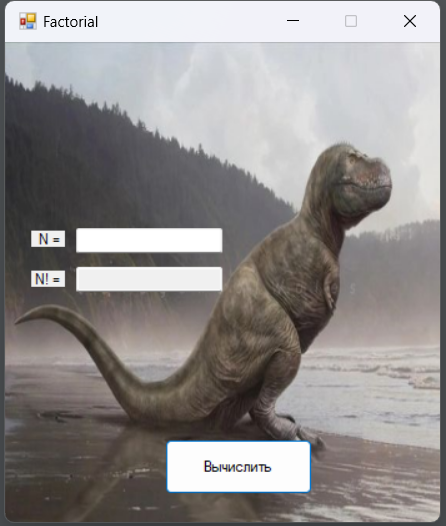
\includegraphics[scale=0.7]{Скрины/Снимок экрана 2025-01-03 193935.png}
    \caption{Окно приложения <<Факториал>> открытое в конструкторе}\label{fig:fact-01}
\end{figure}


У элементов изменены значения некоторых атрибутов. Значения измененных атрибутов представлены в таблице ~\ref{tab:fact-attr}.
\begin{table}[H]
    \small
    \caption{Значения атрибутов элементов в приложении <<Факториал>>}\label{tab:fact-attr}
    \begin{tabular}{|l|l|}\hline
    Наименование атрибута & Значение\cr\hline
    \multicolumn{2}{|l|}{Для формы}\cr\hline
    \verb"Text" & \verb"Factorial"\cr\hline
    \verb"FormBorderStyle" & \verb"Fixed3D"\cr\hline
    \verb"BackgroundImagee" & \verb"System.Drawing.Bitmap"\cr\hline
    \verb"MaximizeBox" & \verb"False"\cr\hline
    \multicolumn{2}{|l|}{Для первой надписи}\cr\hline
    \verb"(Name)" & \verb"lblInput"\cr\hline
    \verb"Text" & \verb" N = "\cr\hline
    \multicolumn{2}{|l|}{Для второй надписи}\cr\hline
    \verb"(Name)" & \verb"lblOutput"\cr\hline
    \verb"Text" & \verb"N! = "\cr\hline
    \multicolumn{2}{|l|}{Для первого текстового поля}\cr\hline
    \verb"(Name)" & \verb"txtInput"\cr\hline
    \multicolumn{2}{|l|}{Для второго текстового поля}\cr\hline
    \verb"(Name)" & \verb"txtOutput"\cr\hline
    \multicolumn{2}{|l|}{Для кнопки}\cr\hline
    \verb"(Name)" & \verb"btnCalculate"\cr\hline
    \verb"Text" & \verb"Вычислить"\cr\hline
    \multicolumn{2}{|l|}{Для обработчика ошибок}\cr\hline
    \verb"(Name)" & \verb"errorProvider"\cr\hline
    \end{tabular}
\end{table}

Была написана функция вычисления факториала:
\inputminted[fontsize=\footnotesize]{cpp}{Код/Fact.cpp}

Здесь переменная \mintinline{cpp}{N} "--- число, для которого нужно вычислить факториал.

На нажатие кнопки <<Вычислить>> установлено выполнение следующего кода:
\inputminted[fontsize=\footnotesize]{cpp}{Код/MyForm1.cpp}

\vspace{10cm}

После запуска приложения на экране появляется окно (см. рисунок~\ref{fig:fact-02}).
\begin{figure}[H]
    \centering
    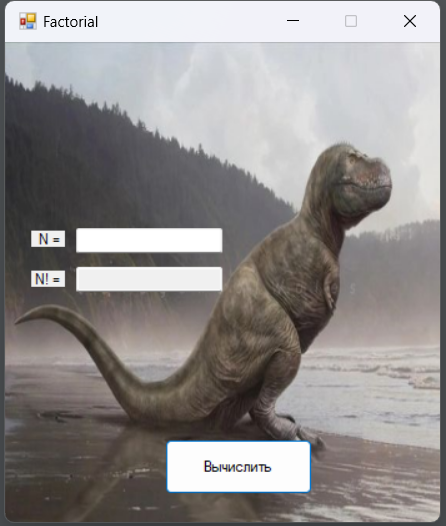
\includegraphics[scale=0.7]{Скрины/Снимок экрана 2025-01-03 193935.png}
    \caption{Окно приложения <<Факториал>>: начальный запуск}\label{fig:fact-02}
\end{figure}

При вводе целого числа после нажатия кнопки в поле вывода приводится результат вычисления факториала для заданного числа (см. рисунок~\ref{fig:fact-03}).

\begin{figure}[H]
    \centering
    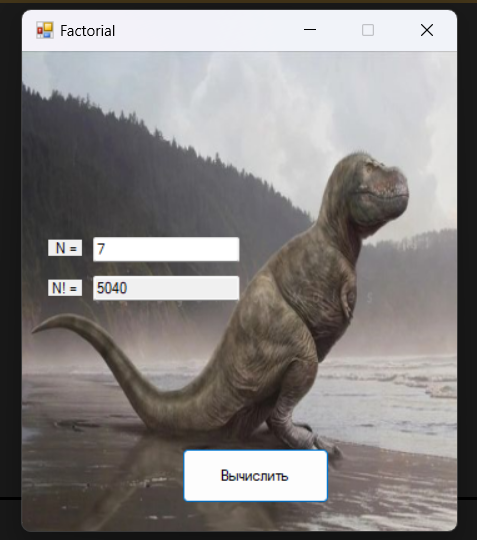
\includegraphics[scale=0.7]{Скрины/Снимок экрана 2025-01-03 203634.png}
    \caption{Окно приложения <<Факториал>>: корректное вычисление}\label{fig:fact-03}
\end{figure}

При вводе некорректного значения возникает сообщение об ошибке (см. рисунок~\ref{fig:fact-04}).
\begin{figure}[H]
    \centering
    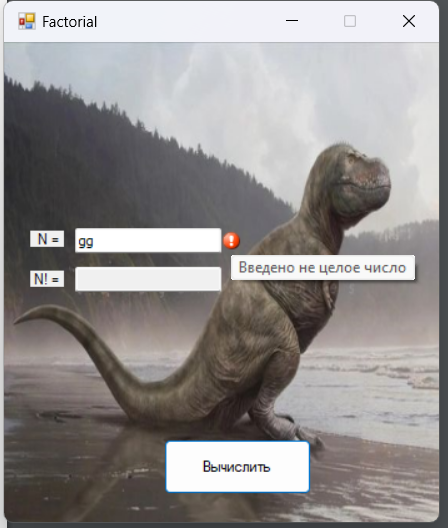
\includegraphics[scale=0.7]{Скрины/Снимок экрана 2025-01-03 203727.png}
    \caption{Окно приложения <<Факториал>>: сообщение о некорректном вводе}\label{fig:fact-04}
\end{figure}

Полный код программы приведен в приложении~\ref{app:CD}.

\section{Простые вычисления}

\textsl{Задание.} Разработать приложение для вычисления значения функции.
Создано окно приложения, содержащее три элемента TextBox, три элемента Label и один элемент Button. Для отображения сообщений об ошибках в
окно добавлены два элемента ErrorProvider. Вид окна представлен на рисунке ~\ref{fig:simple-01}.


\begin{figure}[!ht]
    \centering
    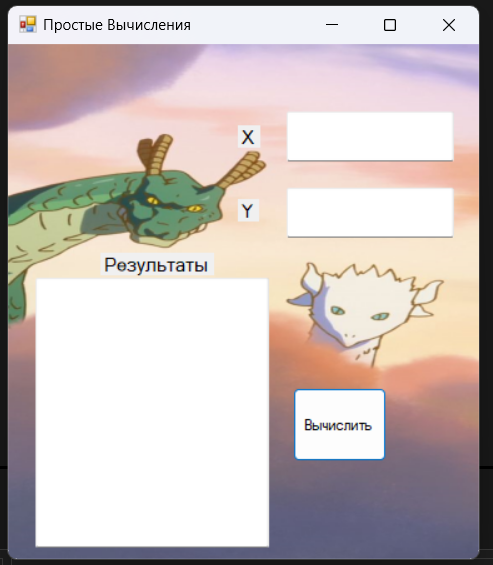
\includegraphics[scale=0.7]{Скрины/Снимок экрана 2025-01-03 212123.png}
    \caption{Окно приложения «Простые вычисления №12» открытое в конструкторе)}\label{fig:simple-01}
\end{figure}


У элементов изменены значения некоторых атрибутов. Значения измененных атрибутов представлены в таблице~\ref{tab:simp-attr}.
\begin{table}[H]
    \small
    \caption{Значения атрибутов элементов в приложении <<Простые вычисления №12>>}\label{tab:simp-attr}
    \begin{tabular}{|l|l|}\hline
    Наименование атрибута & Значение\cr\hline
    \multicolumn{2}{|l|}{Для формы}\cr\hline
    \verb"Text" & \verb"Простые вычисления №7"\cr\hline
    \verb"BackgroundImagee" & \verb"System.Drawing.Bitmap"\cr\hline

    \multicolumn{2}{|l|}{Для первой надписи}\cr\hline
    
    \verb"Text" & \verb"X = "\cr\hline

    \multicolumn{2}{|l|}{Для второй надписи}\cr\hline
   
    \verb"Text" & \verb"Y = "\cr\hline

    \multicolumn{2}{|l|}{Для третьей надписи}\cr\hline
    
    \verb"Text" & \verb"Результаты"\cr\hline

    \multicolumn{2}{|l|}{Для первого текстового поля}\cr\hline
    \verb"(Name)" & \verb"txtInputX"\cr\hline

    \multicolumn{2}{|l|}{Для второго текстового поля}\cr\hline
    \verb"(Name)" & \verb"txtInputY"\cr\hline

    \multicolumn{2}{|l|}{Для третьего текстового поля}\cr\hline
    \verb"(Name)" & \verb"txtOutput"\cr\hline

    \multicolumn{2}{|l|}{Для кнопки}\cr\hline
    \verb"(Name)" & \verb"Calculate"\cr\hline
    \verb"Text" & \verb"Вычислить"\cr\hline
    \end{tabular}
\end{table}

На нажатие кнопки «Вычислить» установлено выполнение следующего
кода:

\inputminted[fontsize=\footnotesize]{cpp}{Код/MyForm2.cpp}

\vspace{10cm}

После запуска приложения на экране появляется окно (см. рисунок~\ref{fig:simple-02}).
\begin{figure}[H]
    \centering
    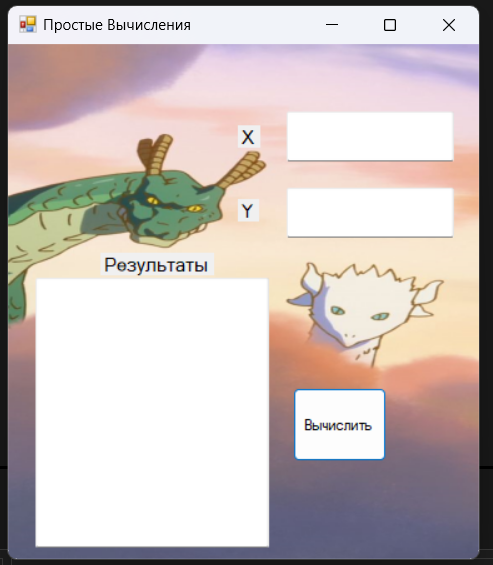
\includegraphics[scale=0.7]{Скрины/Снимок экрана 2025-01-03 212123.png}
    \caption{– Окно приложения «Простые вычисления №12»: начальный запуск}\label{fig:simple-02}
\end{figure}

При вводе целых чисел после нажатия кнопки в поле вывода приводится
результат вычисления функции для заданных чисел (см. рисунок~\ref{fig:simple-03}).

\begin{figure}[H]
    \centering
    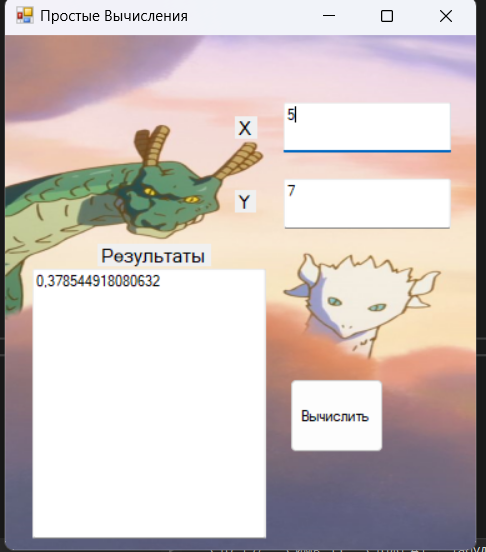
\includegraphics[scale=0.7]{Скрины/Снимок экрана 2025-01-03 215036.png}
    \caption{Окно приложения «Простые вычисления №12»: корректное вычисление}\label{fig:simple-03}
\end{figure}

При вводе некорректного значения возникает сообщение об ошибке (см. рисунки~\ref{fig:simple-04} и ~\ref{fig:simple-05}).

\begin{figure}[H]
    \centering
    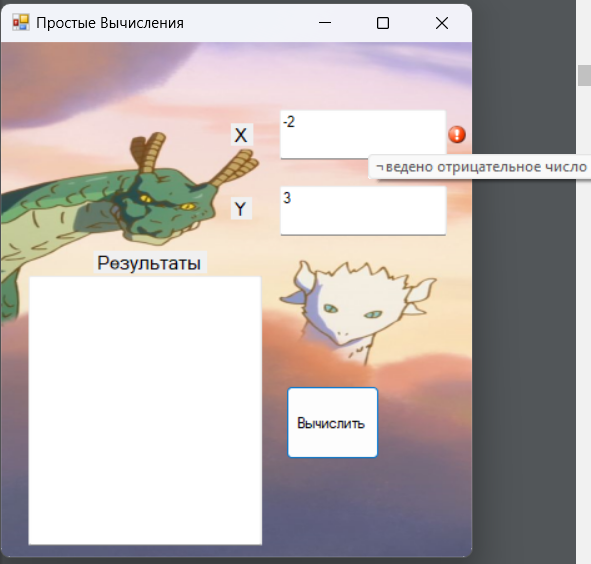
\includegraphics[scale=0.7]{Скрины/Снимок экрана 2025-01-03 215135.png}
    \caption{Окно приложения «Простые вычисления №12»: сообщение о некорректном вводе
(«Введено отрицательное число»)}\label{fig:simple-04}
\end{figure}

\begin{figure}[H]
    \centering
    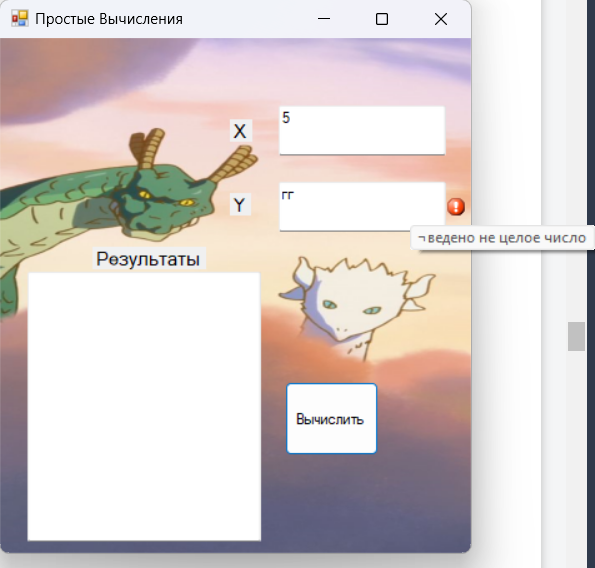
\includegraphics[scale=0.7]{Скрины/Снимок экрана 2025-01-03 215325.png}
    \caption{Окно приложения «Простые вычисления №12»: сообщение о некорректном вводе
(«Введено не число»)}\label{fig:simple-05}
\end{figure}

Полный код программы приведен в приложении~\ref{app:CD}.


\section{Рекурсивные вычисления}

\textsl{Задание.} Разработать приложение для вычисления суммы цифр числа.
Создано окно приложения, содержащее два элемента TextBox, два элемента Label и один элемент Button. Для отображения сообщений об ошибках в окно
добавлен элемент ErrorProvider. Вид окна представлен на рисунке ~\ref{fig:recur-01}.


\begin{figure}[H]
    \centering
    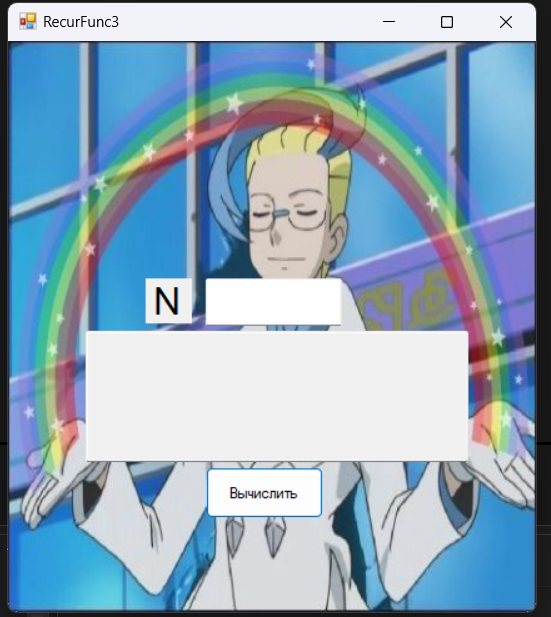
\includegraphics[scale=0.7]{Скрины/Снимок экрана 2025-01-03 220231.png}
    \caption{Окно приложения «RecurFunc3» открытое в конструкторе}\label{fig:recur-01}
\end{figure}


 элементов изменены значения некоторых атрибутов. Значения измененных атрибутов представлены в таблице~\ref{tab:recurs-attr}.
\begin{table}[H]
    \small
    \caption{Значения атрибутов элементов в приложении <<Рекурсия>>}\label{tab:recurs-attr}
    \begin{tabular}{|l|l|}\hline
    Наименование атрибута & Значение\cr\hline
    \multicolumn{2}{|l|}{Для формы}\cr\hline
    \verb"Text" & \verb"Рекурсия"\cr\hline
    \verb"FormBorderStyle" & \verb"Fixed3D"\cr\hline

    \multicolumn{2}{|l|}{Для первой надписи}\cr\hline
    \verb"(Name)" & \verb"lblInput"\cr\hline
    \verb"Text" & \verb"N = "\cr\hline

    \multicolumn{2}{|l|}{Для второй надписи}\cr\hline
    \verb"(Name)" & \verb"lblOutput"\cr\hline
    \verb"Text" & \verb"Результат"\cr\hline

    \multicolumn{2}{|l|}{Для первого текстового поля}\cr\hline
    \verb"(Name)" & \verb"txtInput"\cr\hline

    \multicolumn{2}{|l|}{Для второго текстового поля}\cr\hline
    \verb"(Name)" & \verb"txtOutput"\cr\hline

    \multicolumn{2}{|l|}{Для кнопки}\cr\hline
    \verb"(Name)" & \verb"btnCalc"\cr\hline
    \verb"Text" & \verb"Вычислить"\cr\hline
    \end{tabular}
\end{table}

На нажатие кнопки «Вычислить» установлено выполнение следующего
кода:

\inputminted[fontsize=\footnotesize]{cpp}{Код/RecurFunc3.cpp}



\begin{figure}[H]
    \centering
    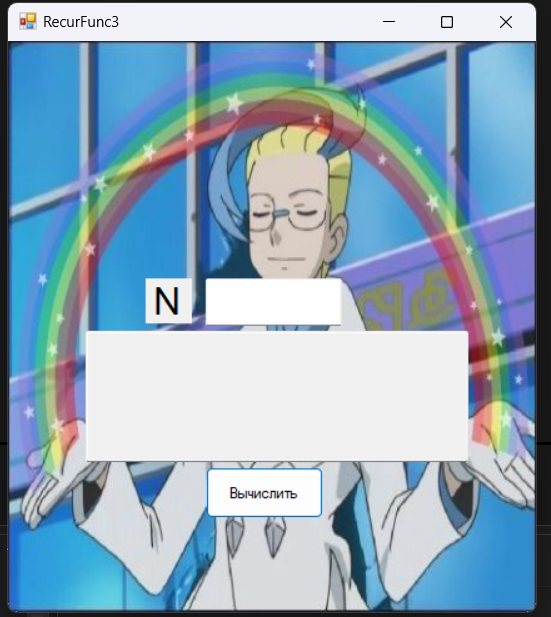
\includegraphics[scale=0.7]{Скрины/Снимок экрана 2025-01-03 220231.png}
    \caption{Окно приложения «RecurFunc3»: начальный запуск}\label{fig:recur-02}
\end{figure}



\begin{figure}[H]
    \centering
    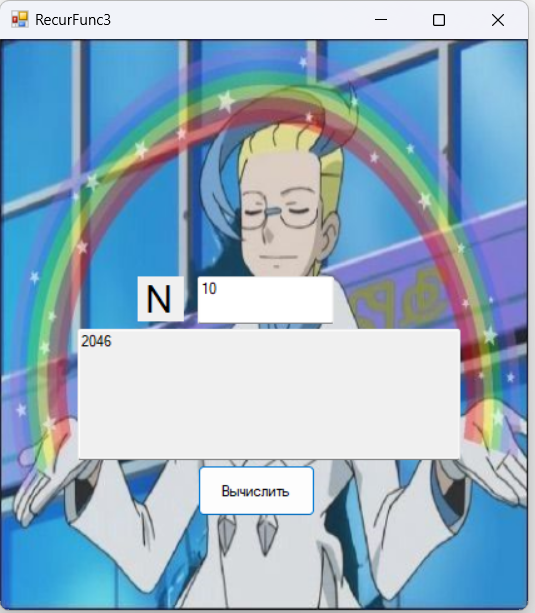
\includegraphics[scale=0.7]{Скрины/Снимок экрана 2025-01-03 221640.png}
    \caption{Окно приложения «RecurFunc3»: корректное вычисление}\label{fig:recur-03}
\end{figure}

При вводе слишком большого значения для вычислений, появляется сообщение о том что происходит переполнение стека ~\ref{fig:recur-04}.

\begin{figure}[H]
    \centering
    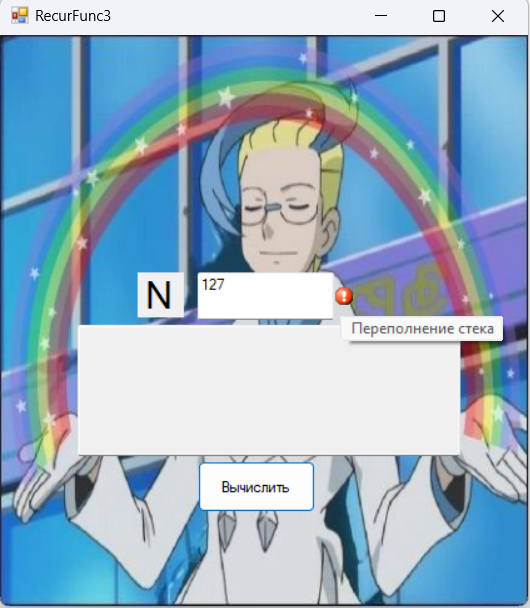
\includegraphics[scale=0.7]{Скрины/Снимок экрана 2025-01-03 221826.png}
    \caption{Окно приложения «RecurFunc3»: некорректное вычисление
    (введение слишком большого значения для вычислений)}\label{fig:recur-04}
\end{figure}

\vspace{11cm}

При вводе некорректного значения возникает сообщение об ошибке (см.
рисунки~\ref{fig:recur-05} и ~\ref{fig:recur-06} ).

\begin{figure}[H]
    \centering
    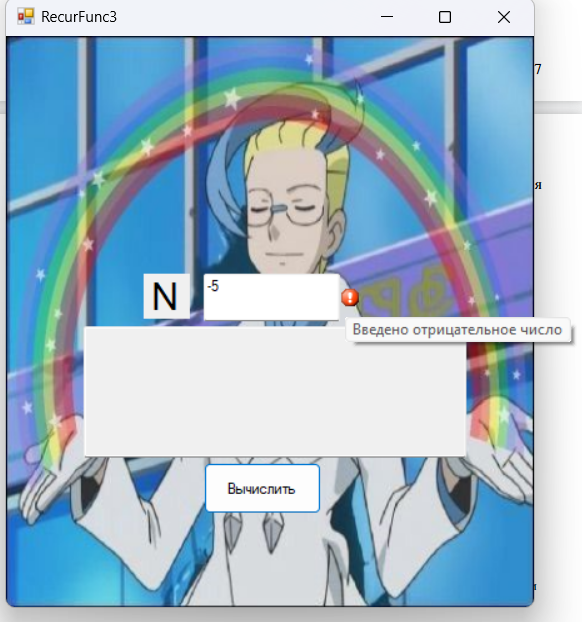
\includegraphics[scale=0.7]{Скрины/Снимок экрана 2025-01-03 222426.png}
    \caption{Окно приложения «RecurFunc3»: некорректное вычисление
    (введение отрицательного числа)}\label{fig:recur-05}
\end{figure}


\begin{figure}[H]
    \centering
    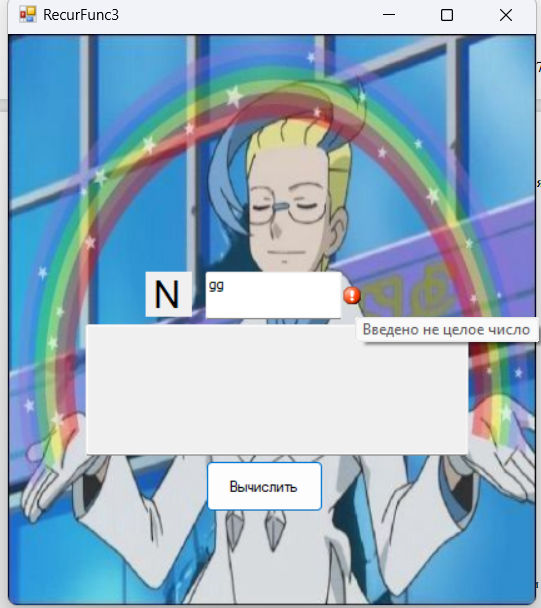
\includegraphics[scale=0.7]{Скрины/Снимок экрана 2025-01-03 222451.png}
    \caption{Окно приложения «RecurFunc3»: некорректное вычисление
    (введение не целого числа)}\label{fig:recur-06}
\end{figure}

Полный код программы приведен в приложении~\ref{app:CD}.



\section{Обработка табличных данных. Часть 1}


\textsl{Задание.} Разработать приложение для работы с одномерным массивом.
Создано окно приложения, содержащее четыре элемента TextBox, пять
элементов Label, четыре элемента Button и один элемент DataGridView\cite{search_5}.
Для отображения сообщений об ошибках в окно добавлены четырые элемента
ErrorProvider. Вид окна представлен на рисунке ~\ref{fig:table1-01}.

\begin{figure}[H]
    \centering
    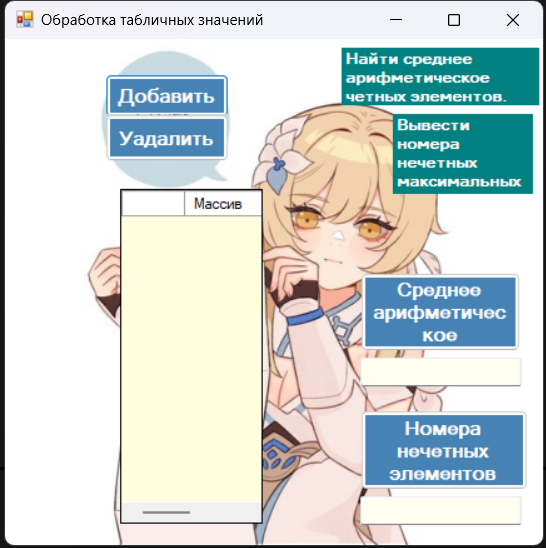
\includegraphics[scale=0.7]{Скрины/Снимок экрана 2025-01-03 222945.png}
    \caption{Окно приложения «Обработка табличных значений»:открытое в конструкторе}\label{fig:table1-01}
\end{figure}


У элементов изменены значения некоторых атрибутов. Значения измененных атрибутов представлены в таблице~\ref{tab:tab1-attr}.
\begin{table}[H]
    \small
    \caption{Значения атрибутов элементов в приложении <<Работа с таблицей>>}\label{tab:tab1-attr}
    \begin{tabular}{|l|l|}\hline
    Наименование атрибута & Значение\cr\hline
    \multicolumn{2}{|l|}{Для формы}\cr\hline
    \verb"Text" & \verb"Обработка табличных данных"\cr\hline

    \multicolumn{2}{|l|}{Для первой надписи}\cr\hline
    \verb"Text" & \verb"Найти среднее арифметическое четных элементов,"\cr\hline

    \multicolumn{2}{|l|}{Для второй надписи}\cr\hline
     \verb"Text" & \verb"Вывести номера нечетных элементов,"\cr\hline
  
    \multicolumn{2}{|l|}{Для первого текстового поля}\cr\hline
    \verb"(Name)" & \verb"SrResult"\cr\hline

    \multicolumn{2}{|l|}{Для второго текстового поля}\cr\hline
    \verb"(Name)" & \verb"NomeraResult"\cr\hline

    \multicolumn{2}{|l|}{Для первой кнопки}\cr\hline
    \verb"(Name)" & \verb"Add"\cr\hline
    \verb"Text" & \verb"Добавить"\cr\hline

    \multicolumn{2}{|l|}{Для второй кнопки}\cr\hline
    \verb"(Name)" & \verb"Delete"\cr\hline
    \verb"Text" & \verb"Удалить"\cr\hline

    \multicolumn{2}{|l|}{Для третьей кнопки}\cr\hline
    \verb"(Name)" & \verb"SredneeArifm"\cr\hline
    \verb"Text" & \verb"Среднее арифмитическое"\cr\hline

    \multicolumn{2}{|l|}{Для четвертой кнопки}\cr\hline
    \verb"(Name)" & \verb"NechotElem"\cr\hline
    \verb"Text" & \verb"Номера неченых элементов"\cr\hline

    \multicolumn{2}{|l|}{Для таблицы}\cr\hline
    \verb"(TextColumn)" & \verb"Массив"\cr\hline
    \end{tabular}
\end{table}

На нажатие кнопки «Добавить» установлено выполнение следующего кода:
\inputminted[fontsize=\footnotesize]{cpp}{Код/Add.cpp}

На нажатие кнопки «Удалить» установлено выполнение следующего кода:
\inputminted[fontsize=\footnotesize]{cpp}{Код/Delete.cpp}

Примеры остальных кодов приведены в приложении~\ref{app:code}.

После запуска приложения на экране появляется окно (см. рисунок ~\ref{fig:table1-02}).

\begin{figure}[H]
    \centering
    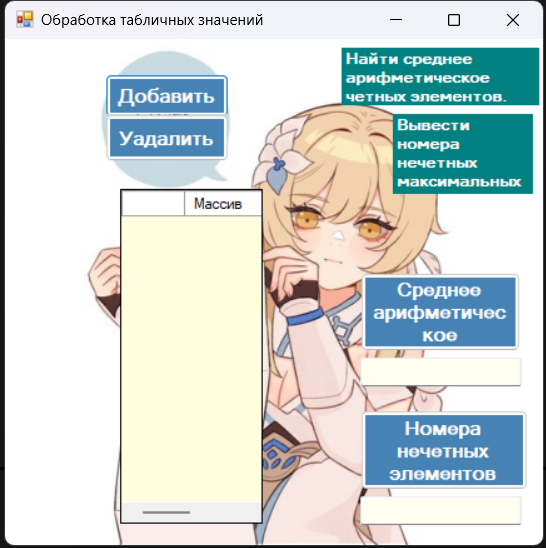
\includegraphics[scale=0.7]{Скрины/Снимок экрана 2025-01-03 222945.png}
    \caption{Окно приложения «Обработка табличных значений»:начальный запуск}\label{fig:table1-02}
\end{figure}

При вводе целых чисел в таблицу и нажатия
кнопки «Среднее арифметическое» в соответствующем поле вывода приводится результат вычисления среднего четных элементов.
При вводе целых чисел в таблицу после нажатия кнопки «Номера нечетных элементов» в соответствующем поле вывода приводится результат вычисления номеров максимальных нечетных элементов (см. рисунок ~\ref{fig:table1-03})

\begin{figure}[H]
    \centering
    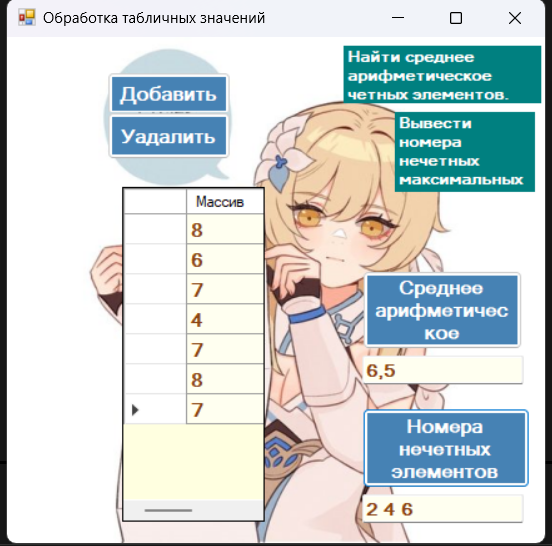
\includegraphics[scale=0.7]{Скрины/Снимок экрана 2025-01-04 235948.png}
    \caption{Окно приложения «Обработка табличных значений»:корректное вычисление}\label{fig:table1-03}
\end{figure}

При вводе некорректного значения возникает сообщение об ошибке (см.
рисунки ~\ref{fig:table1-04} и ~\ref{fig:table1-05}).

\begin{figure}[H]
    \centering
    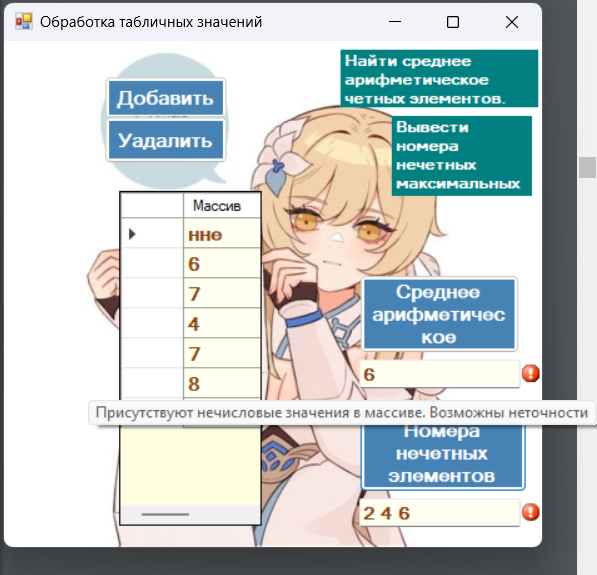
\includegraphics[scale=0.7]{Скрины/Снимок экрана 2025-01-05 000158.png}
    \caption{Окно приложения «Обработка табличных значений»: введение не числа}\label{fig:table1-04}
\end{figure}

\begin{figure}[H]
    \centering
    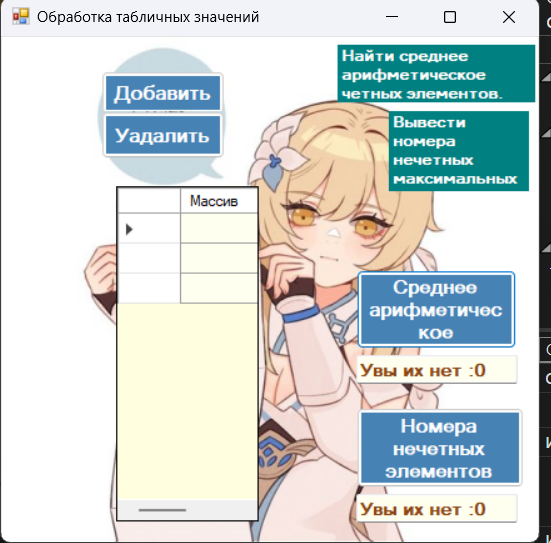
\includegraphics[scale=0.7]{Скрины/Снимок экрана 2025-01-05 000342.png}
    \caption{Окно приложения «Обработка табличных значений»: отсутствие среднего арифметического и номеров нечетных элементов}\label{fig:table1-05}
\end{figure}


Полный код программы приведен в приложении~\ref{app:CD}.

\section{Обработка табличных данных. Часть 2}

\textsl{Задание.} Разработать приложение для работы с двумерным массивом.
Создано окно приложения, два элемента Label, пять элементов Button и два элемент DataGridView, один элемент PictureBox. Для отображения
сообщений об ошибках в окно добавлены два элемента ErrorProvider. Вид окна
представлен на рисунке ~\ref{fig:table2-01}.

\begin{figure}[H]
    \centering
    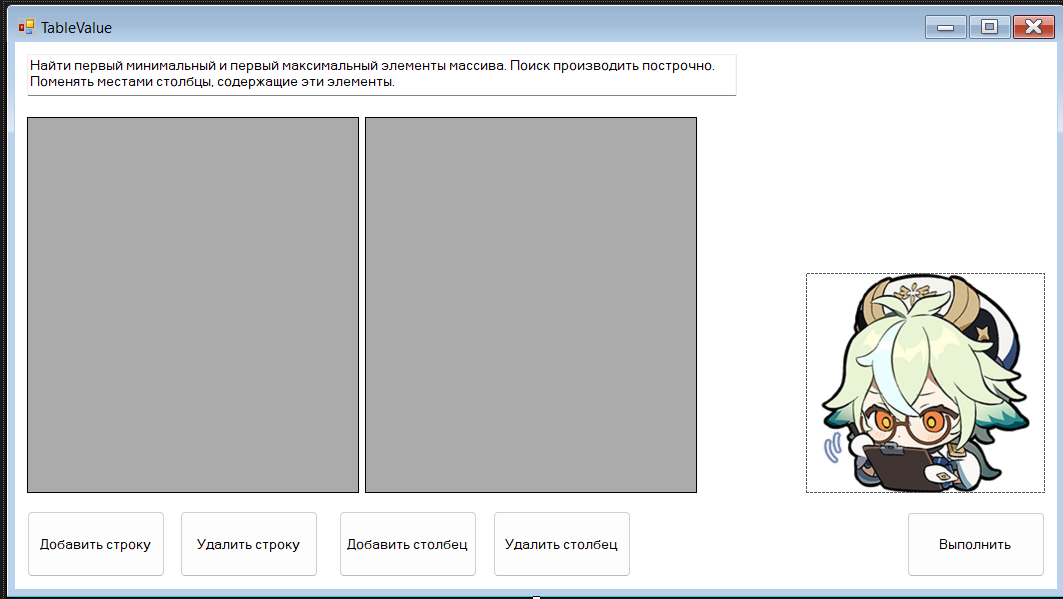
\includegraphics[scale=0.5]{Скрины/Снимок экрана 2025-01-05 114416.png}
    \caption{Окно приложения «TableValue» открытое в
конструкторе)}\label{fig:table2-01}
\end{figure}

У элементов изменены значения некоторых атрибутов. Значения измененных атрибутов представлены в таблице~\ref{tab:tab2-attr}

\begin{table}[H]
    \small
    \caption{Значения атрибутов элементов в приложении <<TableValue>>}\label{tab:tab2-attr}
    \begin{tabular}{|l|l|}\hline
    Наименование атрибута & Значение\cr\hline
    \multicolumn{2}{|l|}{Для формы}\cr\hline
    \verb"Text" & \verb"TableValue"\cr\hline

    \multicolumn{2}{|l|}{Для первой надписи}\cr\hline
    \verb"(Name)" & \verb"Task"\cr\hline
    \verb"Text" & \verb"Найти первый минимальный и первый максимальный"\\ 
    &\verb"элементы массива."\\ 
    &\verb"Поиск производить построчно."\\ 
     &\verb"Поменять местами столбцы, содержащие эти элементы."\cr\hline

    \multicolumn{2}{|l|}{Для первой кнопки}\cr\hline
    \verb"(Name)" & \verb"AddString"\cr\hline
    \verb"Text" & \verb"Добавить строку"\cr\hline

    \multicolumn{2}{|l|}{Для второй кнопки}\cr\hline
    \verb"(Name)" & \verb"DeleteString"\cr\hline
    \verb"Text" & \verb"Удалить строку"\cr\hline

    \multicolumn{2}{|l|}{Для третьей кнопки}\cr\hline
    \verb"(Name)" & \verb"AddColumn"\cr\hline
    \verb"Text" & \verb"Добавить столбец"\cr\hline

    \multicolumn{2}{|l|}{Для четвертой кнопки}\cr\hline
    \verb"(Name)" & \verb"DeleteColumn"\cr\hline
    \verb"Text" & \verb"Удалить столбец"\cr\hline

    \multicolumn{2}{|l|}{Для пятой кнопки}\cr\hline
    \verb"(Name)" & \verb"Execute"\cr\hline
    \verb"Text" & \verb"Выполнить"\cr\hline

    \multicolumn{2}{|l|}{Для первой таблицы}\cr\hline
    \verb"(Name)" & \verb"DataMassivInPut"\cr\hline

    \multicolumn{2}{|l|}{Для второй таблицы}\cr\hline
    \verb"(Name)" & \verb"DataMassivOutPut"\cr\hline
    \end{tabular}
\end{table}

На нажатие кнопки «Добавить строку» установлено выполнение следующего кода:\inputminted[fontsize=\footnotesize]{cpp}{КодТаблица2/AddSrtring.cpp}

На нажатие кнопки «Удалить строку» установлено выполнение следующего кода:\inputminted[fontsize=\footnotesize]{cpp}{КодТаблица2/DeleteString.cpp}

На нажатие кнопки «Добавить столбец» установлено выполнение следующего кода:\inputminted[fontsize=\footnotesize]{cpp}{КодТаблица2/AddCol.cpp}

На нажатие кнопки «Удалить столбец» установлено выполнение следующего кода:\inputminted[fontsize=\footnotesize]{cpp}{КодТаблица2/DeleteCol.cpp}



Примеры остальных кодов приведены в приложении~\ref{app:code}.

После запуска приложения на экране появляется окно (см. рисунок ~\ref{fig:table2-02}).

\begin{figure}[H]
    \centering
    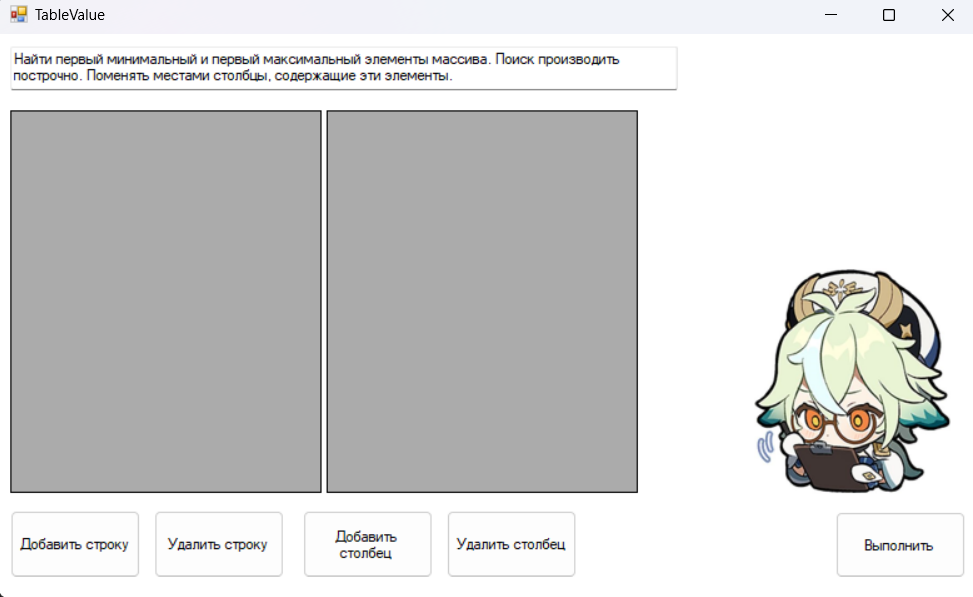
\includegraphics[scale=0.5]{Скрины/Снимок экрана 2025-01-05 121321.png}
    \caption{Окно приложения «TableValue» открытое в
конструкторе}\label{fig:table2-02}
\end{figure}

При вводе целых чисел в первую таблицу после нажатия кнопки «Выполнить» во второй таблице приводится результат замены столбцов содержащих первый минимальный и первый максимальный элементы массива  (см. рисунок ~\ref{fig:table2-03}).

\begin{figure}[H]
    \centering
    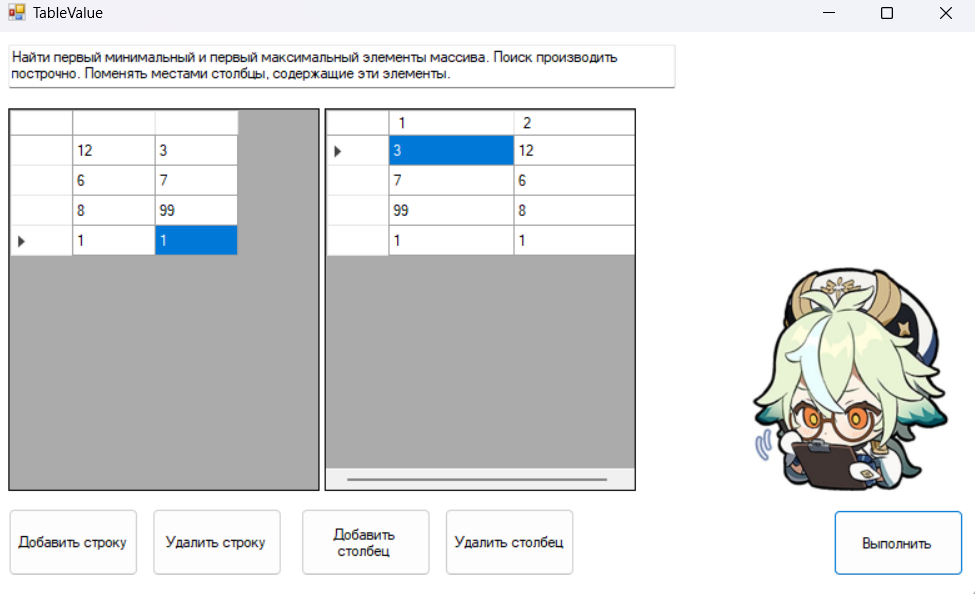
\includegraphics[scale=0.5]{Скрины/Снимок экрана 2025-01-05 121530.png}
    \caption{Окно приложения «TableValue»: корректное вычисление}\label{fig:table2-03}
\end{figure}

При вводе некорректного значения возникает сообщение об ошибке (см.
рисунки ~\ref{fig:table2-04} и  ~\ref{fig:table2-05}).

\begin{figure}[H]
    \centering
    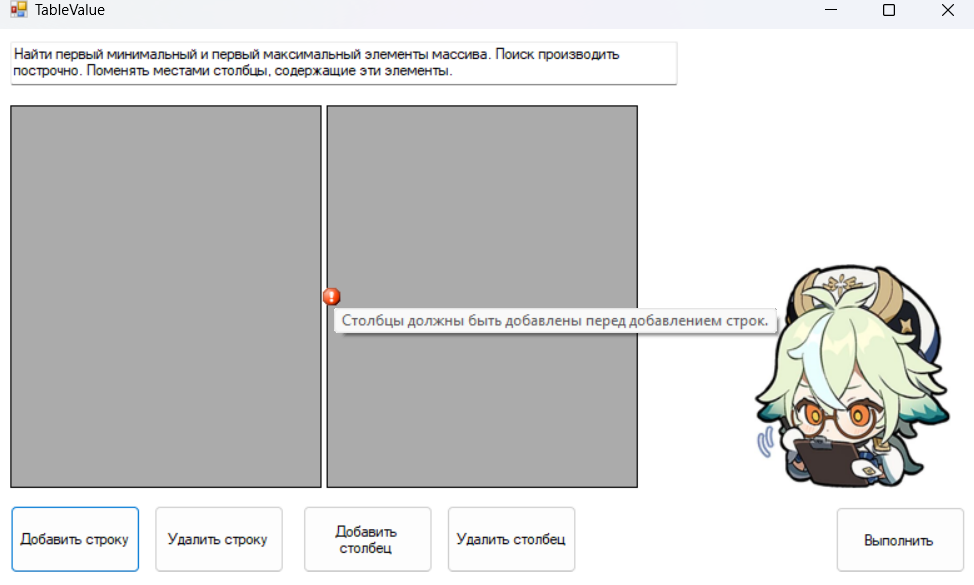
\includegraphics[scale=0.5]{Скрины/Снимок экрана 2025-01-05 121940.png}
    \caption{Окно приложения «TableValue» некорректный ввод (Столбцы должны быть добавлены перед добавлением строк.)}\label{fig:table2-04}
\end{figure}

\begin{figure}[H]
    \centering
    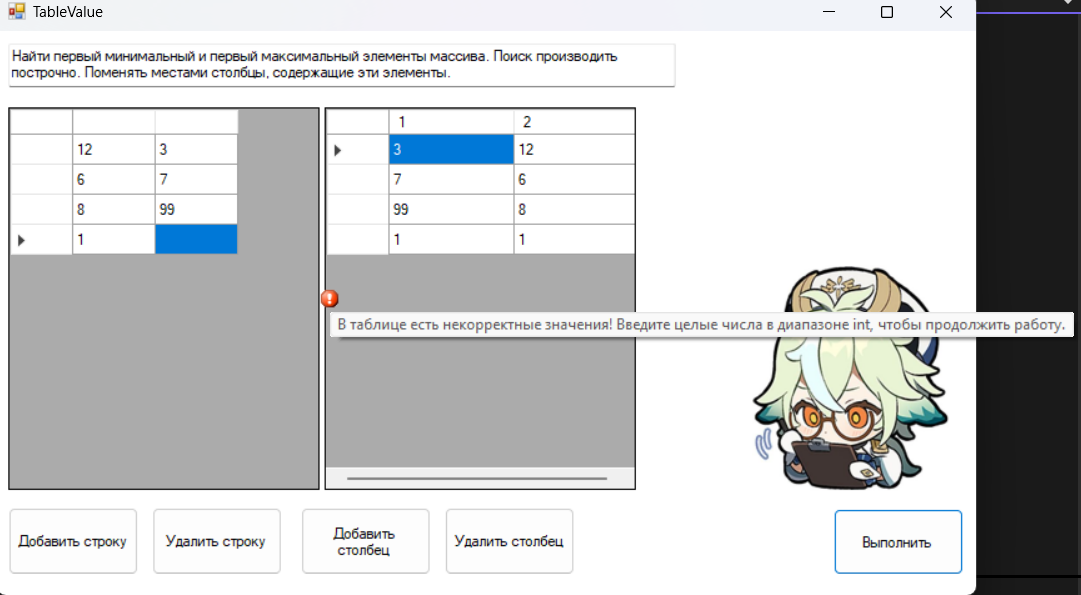
\includegraphics[scale=0.5]{Скрины/Снимок экрана 2025-01-05 121857.png}
    \caption{Окно приложения «TableValue» некорректный ввод (В таблице есть некорректные значения! Введите целые числа в диапазоне int, чтобы продолжить работу.)}\label{fig:table2-05}
\end{figure}


Полный код программы приведен в приложении~\ref{app:CD}.

\section{Матричный калькулятор}

\textsl{Задание.} Разработать приложение «Матричный калькулятор»\cite{search_6}.
Создано окно приложения, содержащее три элемента TextBox, семь элементов Label, семнадцать элементов Button, пять элемент DataGridView, один элемент PictureBox, один элемент GroupBox и четырнадцать элементов RadioButton. Для отображения сообщений об ошибках в окно добавлены восемь элементов ErrorProvider. Вид окна
представлен на рисунке ~\ref{fig:matrix-01}.


\begin{figure}[H]
    \centering
    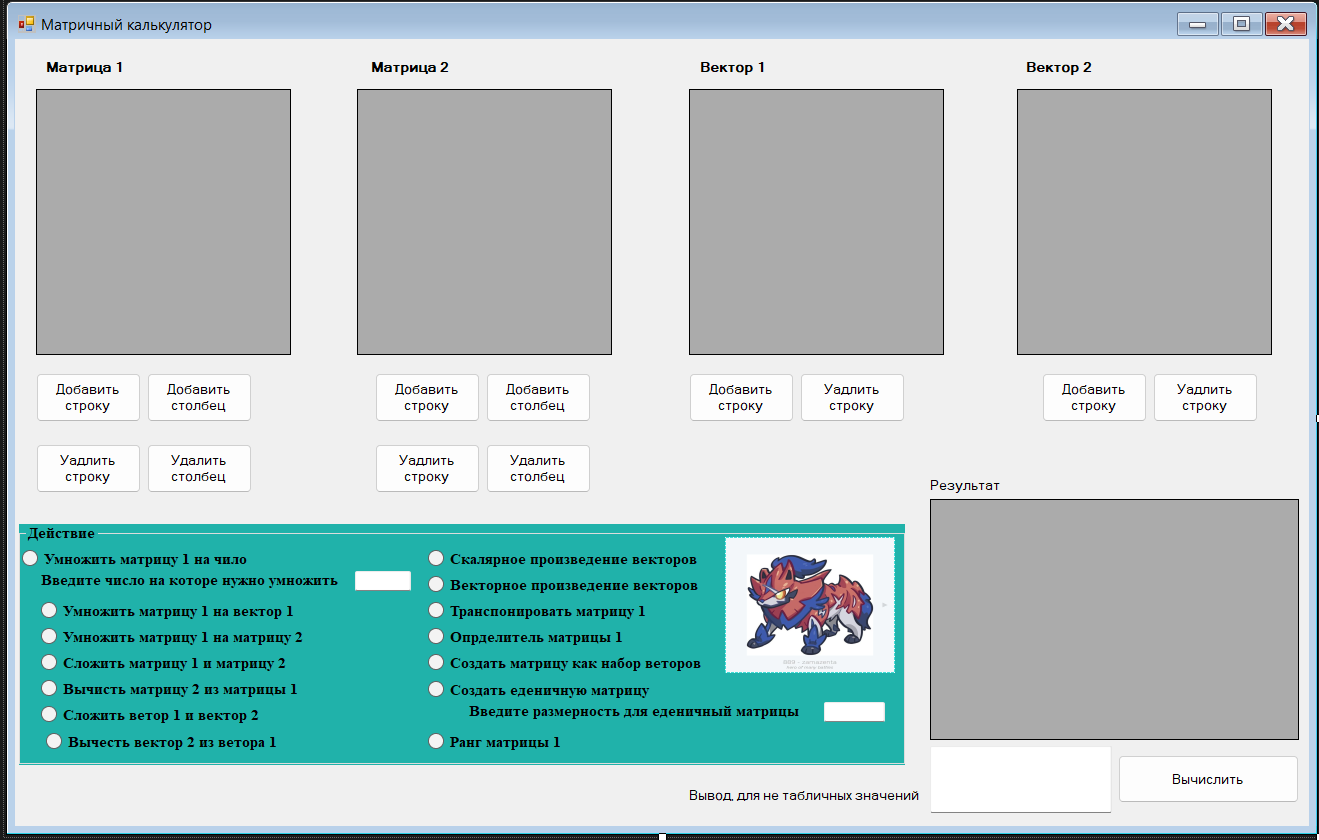
\includegraphics[scale=0.5]{Скрины/Снимок экрана 2025-01-05 123032.png}
    \caption{Окно приложения «Матричный калькулятор» открытое в конструкторе}\label{fig:matrix-01}
\end{figure}


У элементов изменены значения некоторых атрибутов. Значения измененных атрибутов представлены в таблицах~\ref{tab:tab3-1-attr}, ~\ref{tab:tab3-2-attr}, ~\ref{tab:tab3-3-attr} и ~\ref{tab:tab3-4-attr}.

\begin{table}[H]
    \small
    \caption{Значения атрибутов элементов в приложении <<Матричный калькулятор>>}\label{tab:tab3-1-attr}
    \begin{tabular}{|l|l|}\hline
    Наименование атрибута & Значение\cr\hline
    \multicolumn{2}{|l|}{Для формы}\cr\hline
    \verb"Text" & \verb"Матричный калькулятор"\cr\hline

    \multicolumn{2}{|l|}{Для первой надписи}\cr\hline
    \verb"Text" & \verb"Матрица 1"\cr\hline

    \multicolumn{2}{|l|}{Для второй надписи}\cr\hline
    \verb"Text" & \verb"Матрица 2"\cr\hline
    \end{tabular}
\end{table}

\begin{table}[H]
    \small
    \caption{Значения атрибутов элементов в приложении <<Матричный калькулятор>>}\label{tab:tab3-2-attr}
    \begin{tabular}{|l|l|}\hline
    Наименование атрибута & Значение\cr\hline

    \multicolumn{2}{|l|}{Для третьей надписи}\cr\hline
    \verb"Text" & \verb"Вектор 1"\cr\hline

    \multicolumn{2}{|l|}{Для четвертой надписи}\cr\hline
    \verb"Text" & \verb"Вектор 2"\cr\hline

    \multicolumn{2}{|l|}{Для пятой надписи}\cr\hline
    \verb"Text" & \verb"Введите размерерность для еденичной матрицы: "\cr\hline

    \multicolumn{2}{|l|}{Для шестой надписи}\cr\hline
    \verb"Text" & \verb"Результат"\cr\hline

    \multicolumn{2}{|l|}{Для седьмой надписи}\cr\hline
    \verb"Text" & \verb"Вывод, для не табличных значений"\cr\hline

    \multicolumn{2}{|l|}{Для первого текстового поля}\cr\hline
    \verb"(Name)" & \verb"InPutNumber"\cr\hline

    \multicolumn{2}{|l|}{Для второго текстового поля}\cr\hline
    \verb"(Name)" & \verb"MatrixSize"\cr\hline

    \multicolumn{2}{|l|}{Для третьего текстового поля}\cr\hline
    \verb"(Name)" & \verb"ResultText"\cr\hline

    \multicolumn{2}{|l|}{Для первой кнопки}\cr\hline
    \verb"(Name)" & \verb"AddString"\cr\hline
    \verb"Text" & \verb"Добавить строку"\cr\hline

    \multicolumn{2}{|l|}{Для второй кнопки}\cr\hline
    \verb"(Name)" & \verb"DeleteString"\cr\hline
    \verb"Text" & \verb"Удалить строку"\cr\hline

    \multicolumn{2}{|l|}{Для третьей кнопки}\cr\hline
    \verb"(Name)" & \verb"AddColumn"\cr\hline
    \verb"Text" & \verb"Добавить столбец"\cr\hline

    \multicolumn{2}{|l|}{Для четвертой кнопки}\cr\hline
    \verb"(Name)" & \verb"DeleteColumn"\cr\hline
    \verb"Text" & \verb"Удалить столбец"\cr\hline


    \multicolumn{2}{|l|}{Для пятой кнопки}\cr\hline
    \verb"(Name)" & \verb"AddString2"\cr\hline
    \verb"Text" & \verb"Добавить строку"\cr\hline

    \multicolumn{2}{|l|}{Для шестой кнопки}\cr\hline
    \verb"(Name)" & \verb"DeleteString2"\cr\hline
    \verb"Text" & \verb"Удалить строку"\cr\hline

    \multicolumn{2}{|l|}{Для седьмой кнопки}\cr\hline
    \verb"(Name)" & \verb"AddColumn2"\cr\hline
    \verb"Text" & \verb"Добавить столбец"\cr\hline

    \multicolumn{2}{|l|}{Для восьмой кнопки}\cr\hline
    \verb"(Name)" & \verb"DeleteColumn2"\cr\hline
    \verb"Text" & \verb"Удалить столбец"\cr\hline
    
    \end{tabular}
\end{table}

\begin{table}[H]
    \small
    \caption{Значения атрибутов элементов в приложении <<Матричный калькулятор>>}\label{tab:tab3-3-attr}
    \begin{tabular}{|l|l|}\hline
    Наименование атрибута & Значение\cr\hline
    
    \multicolumn{2}{|l|}{Для девятой кнопки}\cr\hline
    \verb"(Name)" & \verb"AddStringV"\cr\hline
    \verb"Text" & \verb"Добавить строку"\cr\hline

    \multicolumn{2}{|l|}{Для десятой кнопки}\cr\hline
    \verb"(Name)" & \verb"DeleteStringV"\cr\hline
    \verb"Text" & \verb"Удалить строку"\cr\hline

 
    \multicolumn{2}{|l|}{Для одиннадцатой кнопки}\cr\hline
    \verb"(Name)" & \verb"AddStringV2"\cr\hline
    \verb"Text" & \verb"Добавить строку"\cr\hline

    \multicolumn{2}{|l|}{Для двенадцатой кнопки}\cr\hline
    \verb"(Name)" & \verb"DeleteStringV2"\cr\hline
    \verb"Text" & \verb"Удалить строку"\cr\hline

  
    \multicolumn{2}{|l|}{Для тринадцатой кнопки}\cr\hline
    \verb"(Name)" & \verb"btnCalc"\cr\hline
    \verb"Text" & \verb"Execute"\cr\hline

    \multicolumn{2}{|l|}{Для первой таблицы}\cr\hline
    \verb"(Name)" & \verb"Matrix1"\cr\hline

    \multicolumn{2}{|l|}{Для второй таблицы}\cr\hline
    \verb"(Name)" & \verb"Matrix2"\cr\hline

    \multicolumn{2}{|l|}{Для третьей таблицы}\cr\hline
    \verb"(Name)" & \verb"Vector1"\cr\hline

    \multicolumn{2}{|l|}{Для четвертой таблицы}\cr\hline
    \verb"(Name)" & \verb"Vector2"\cr\hline

    \multicolumn{2}{|l|}{Для пятой таблицы}\cr\hline
    \verb"(Name)" & \verb"Result"\cr\hline

    \multicolumn{2}{|l|}{Для группового окна}\cr\hline
    \verb"Text" & \verb"Действия"\cr\hline

    \end{tabular}
\end{table}

\begin{table}[H]
    \small
    \caption{Значения атрибутов элементов в приложении <<Матричный калькулятор>>}\label{tab:tab3-4-attr}
    \begin{tabular}{|l|l|}\hline
    Наименование атрибута & Значение\cr\hline

    \multicolumn{2}{|l|}{Для первого переключателя}\cr\hline
    \verb"(Name)" & \verb"multX"\cr\hline
    \verb"Text" & \verb"Умножить первую матрицу на число"\cr\hline

    \multicolumn{2}{|l|}{Для второго переключателя}\cr\hline
    \verb"(Name)" & \verb"multVect"\cr\hline
    \verb"Text" & \verb"Умножить первую матрицу на первый вектор"\cr\hline

    \multicolumn{2}{|l|}{Для третьего переключателя}\cr\hline
    \verb"(Name)" & \verb"multMatr"\cr\hline
    \verb"Text" & \verb"Умножить первую матрицу на вторую матрицу"\cr\hline

    \multicolumn{2}{|l|}{Для четвертого переключателя}\cr\hline
    \verb"(Name)" & \verb"plusMatr"\cr\hline
    \verb"Text" & \verb"Сложить две матрицы"\cr\hline

    \multicolumn{2}{|l|}{Для пятого переключателя}\cr\hline
    \verb"(Name)" & \verb"minusMatr"\cr\hline
    \verb"Text" & \verb"Вычесть из первой матрицы вторую матрицу"\cr\hline

    \multicolumn{2}{|l|}{Для шестого переключателя}\cr\hline
    \verb"(Name)" & \verb"plusVect"\cr\hline
    \verb"Text" & \verb"Сложить два вектора"\cr\hline

    \multicolumn{2}{|l|}{Для седьмого переключателя}\cr\hline
    \verb"(Name)" & \verb"minusVect"\cr\hline
    \verb"Text" & \verb"Вычесть из первого вектора второй вектор"\cr\hline

    \multicolumn{2}{|l|}{Для восьмого переключателя}\cr\hline
    \verb"(Name)" & \verb"skalMultVect"\cr\hline
    \verb"Text" & \verb"Скалярное произведение двух векторов"\cr\hline

    \multicolumn{2}{|l|}{Для девятого переключателя}\cr\hline
    \verb"(Name)" & \verb"vectMultVect"\cr\hline
    \verb"Text" & \verb"Векторное произведение двух векторов"\cr\hline

    \multicolumn{2}{|l|}{Для десятого переключателя}\cr\hline
    \verb"(Name)" & \verb"transMatr"\cr\hline
    \verb"Text" & \verb"Транспонирование первой матрицы"\cr\hline

    \multicolumn{2}{|l|}{Для одиннадцатого переключателя}\cr\hline
    \verb"(Name)" & \verb"OpredRangMatr"\cr\hline
    \verb"Text" & \verb"Определитель"\cr\hline

    \multicolumn{2}{|l|}{Для двенадцатого переключателя}\cr\hline
    \verb"(Name)" & \verb"createMatrVect"\cr\hline
    \verb"Text" & \verb"Создать матрицу как набор векторов"\cr\hline

    \multicolumn{2}{|l|}{Для тринадцатого переключателя}\cr\hline
    \verb"(Name)" & \verb"edinMatr"\cr\hline
    \verb"Text" & \verb"Создать единичную матрицу"\cr\hline

    \end{tabular}
\end{table}  


На нажатие кнопки <<Добавить строку>> установлено выполнение следующего кода:
\inputminted[fontsize=\footnotesize]{cpp}{КодМатрикс/AddString.cpp}

На нажатие кнопки <<Удалить строку>> установлено выполнение следующего кода:
\inputminted[fontsize=\footnotesize]{cpp}{КодМатрикс/DeleteString.cpp}

На нажатие кнопки <<Добавить столбец>> установлено выполнение следующего кода:
\inputminted[fontsize=\footnotesize]{cpp}{КодМатрикс/AddCol.cpp}

На нажатие кнопки <<Удалить столбец>> установлено выполнение следующего кода:
\inputminted[fontsize=\footnotesize]{cpp}{КодМатрикс/Deletezcol.cpp}

Примеры остальных кодов приведены в приложении~\ref{app:code}.

После запуска приложения на экране появляется окно (см.рисунок ~\ref{fig:matrix-02}).

\begin{figure}[H]
    \centering
    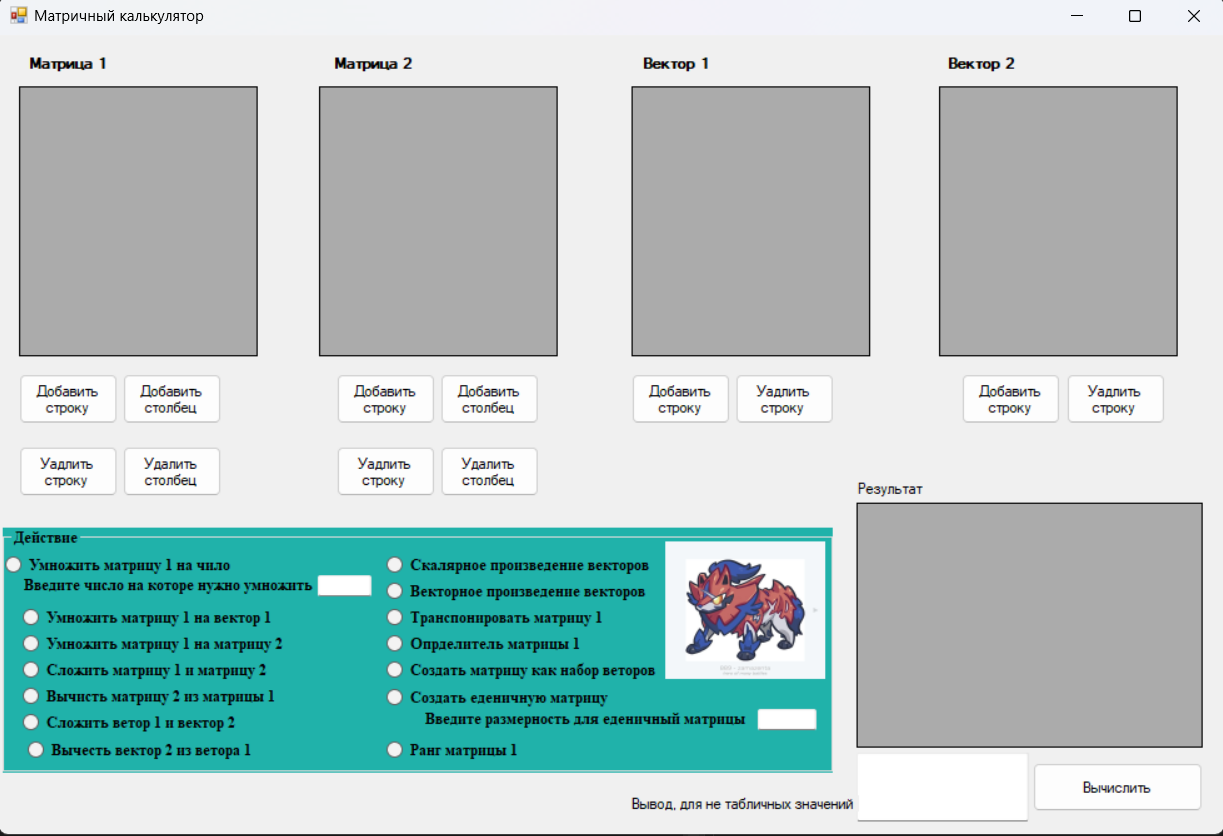
\includegraphics[scale=0.4]{Скрины/Снимок экрана 2025-01-05 131634.png}
    \caption{Окно приложения <<Матричный калькулятор>>: начальный запуск}\label{fig:matrix-02}
\end{figure}

При нажатии на кнопку <<Добавить столбец>> под первой таблицей в ней добавляется пустой столбец (см. рисунок~\ref{fig:matrix-03}).

\begin{figure}[H]
    \centering
    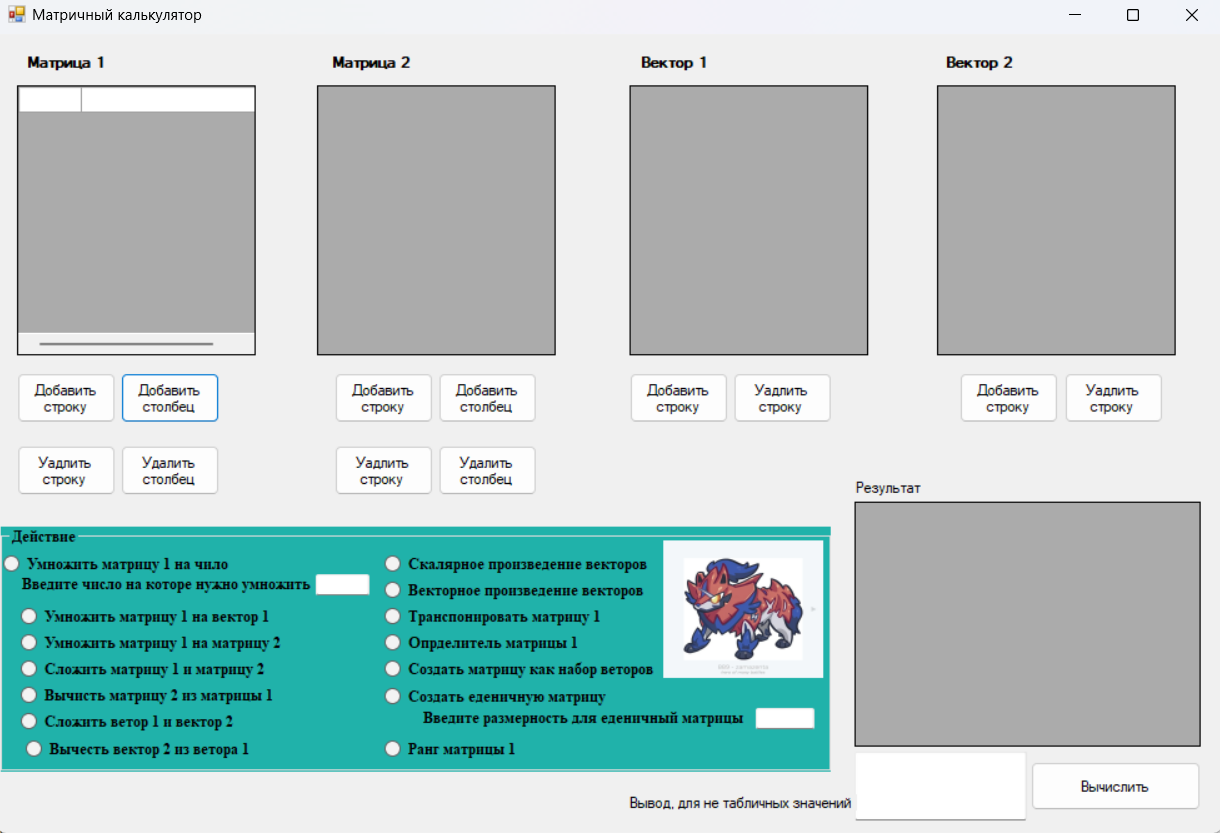
\includegraphics[scale=0.4]{Скрины/Снимок экрана 2025-01-05 131707.png}
    \caption{Окно приложения <<Матричный калькулятор>>: корректное добавление столбца}\label{fig:matrix-03}
\end{figure}

При нажатии на кнопку <<Удалить столбец>> под первой таблицей из нее удаляется выбранный столбец (см. рисунок~\ref{fig:matrix-04}).

\begin{figure}[H]
    \centering
    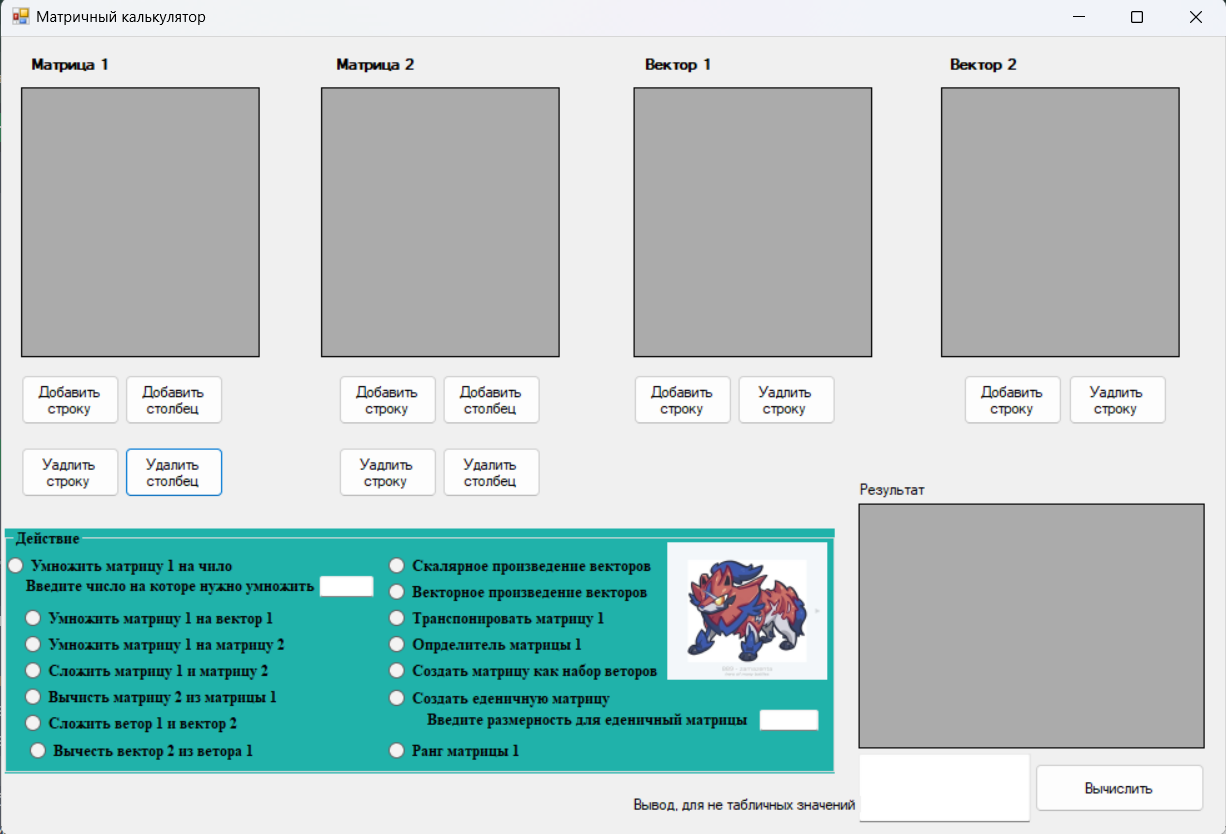
\includegraphics[scale=0.4]{Скрины/Снимок экрана 2025-01-05 131744.png}
    \caption{Окно приложения <<Матричный калькулятор>>: корректное удаление столбца}\label{fig:matrix-04}
\end{figure}


При выборе переключателя <<Скалярное произведение векторов>> и нажатия на кнопку <<Вычислить>> в третье текстовое поле записывается результат (см. рисунок ~\ref{fig:matrix-08}).

\begin{figure}[H]
    \centering
    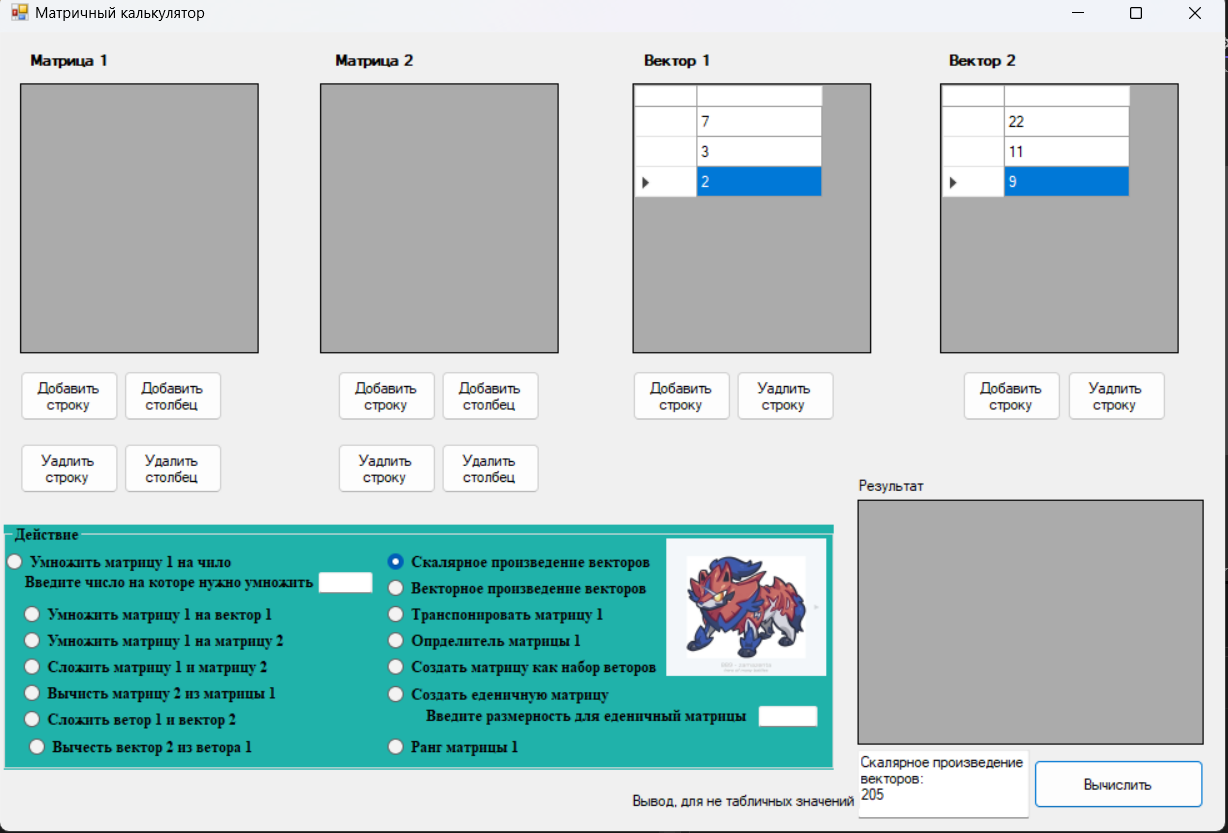
\includegraphics[scale=0.4]{Скрины/Снимок экрана 2025-01-05 133451.png}
    \caption{Окно приложения <<Матричный калькулятор>>: корректное вычисление скалярного произведения векторов}\label{fig:matrix-08}
\end{figure}

При выборе переключателя <<Создать единичную матрицу>> и вводе во второе текстовое поле целого числа после нажатия на кнопку <<Вычислить>> в пятую таблицу записывается результат создания единичной матрицы с размерностью заданного числа (см. рисунок~\ref{fig:matrix-05}).

\begin{figure}[H]
    \centering
    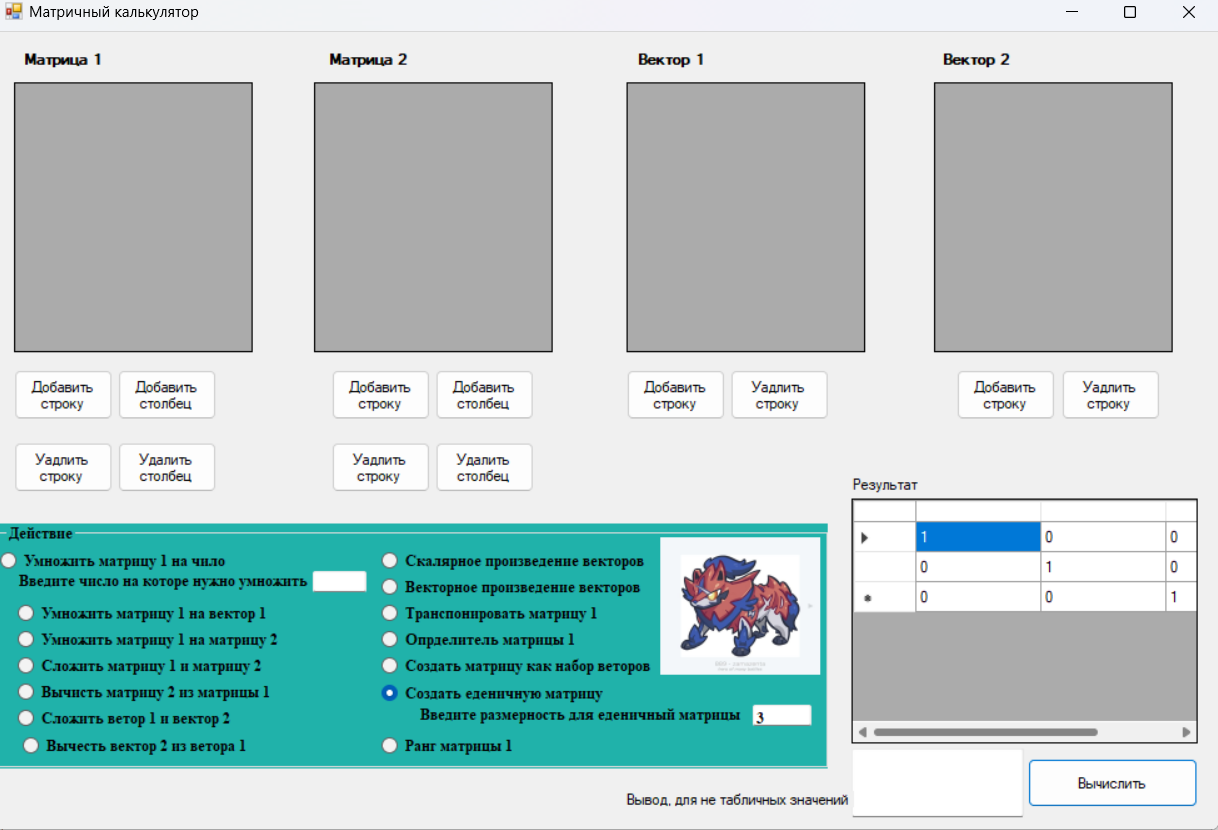
\includegraphics[scale=0.4]{Скрины/Снимок экрана 2025-01-05 131824.png}
    \caption{Окно приложения <<Матричный калькулятор>>: корректное создание единичной матрицы}\label{fig:matrix-05}
\end{figure}

При выборе переключателя <<Умножить первую матрицу на число>> и нажатия кнопке <<Вычислить>> значения матрица изменяются и результат записывается в пятую таблица  (см. рисунок~\ref{fig:matrix-06}).



\begin{figure}[H]
    \centering
    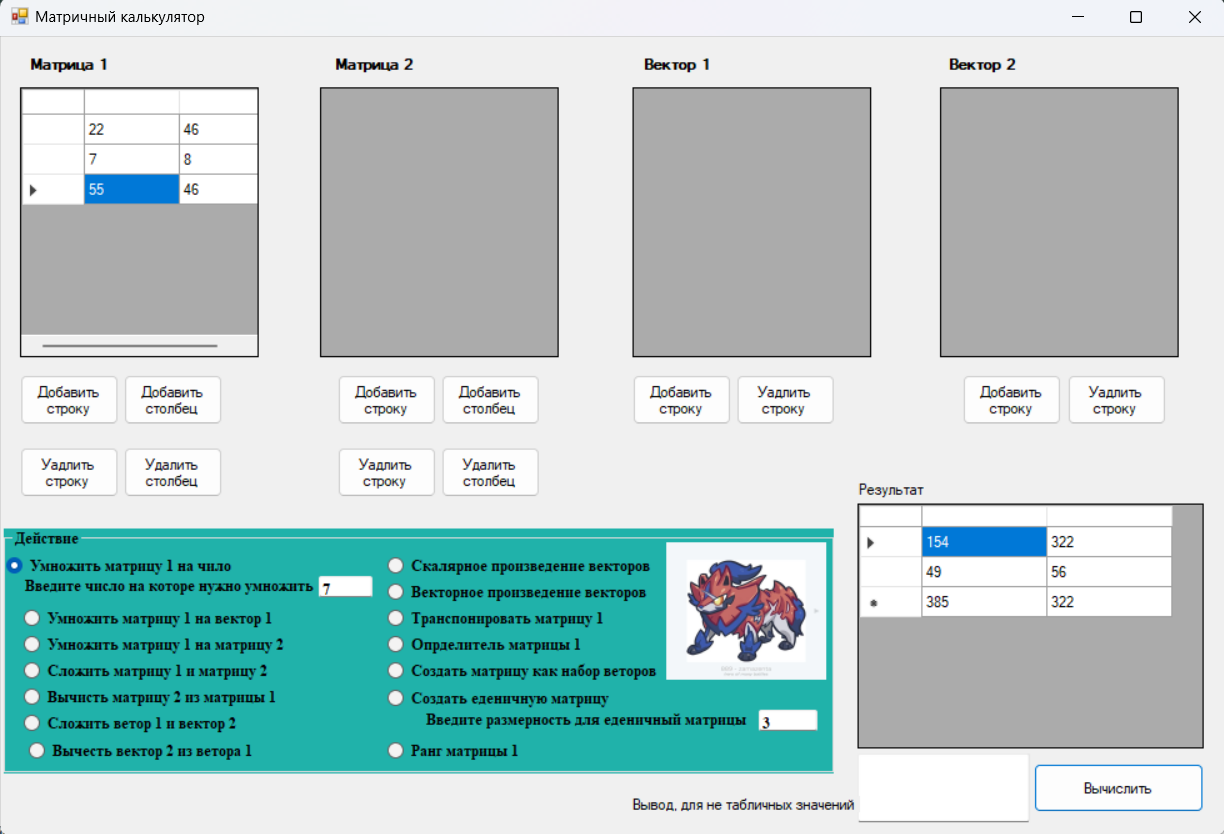
\includegraphics[scale=0.4]{Скрины/Снимок экрана 2025-01-05 132152.png}
    \caption{Окно приложения <<Матричный калькулятор>>: корректное умножение на число}\label{fig:matrix-06}
\end{figure}

При выборе переключателя <<Определитель>> и создании не квадратной матрицы возникает сообщение об ошибке (см. рисунок~\ref{fig:matrix-07}).

\begin{figure}[H]
    \centering
    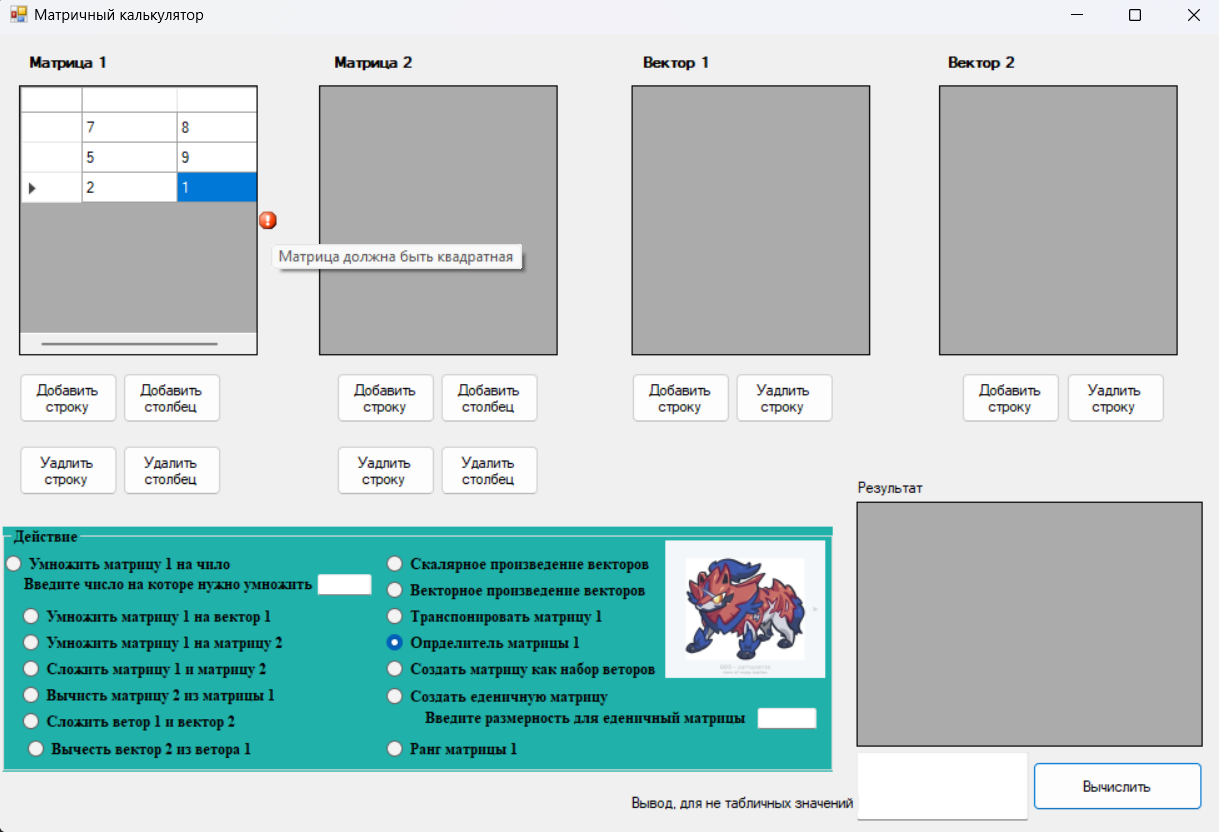
\includegraphics[scale=0.4]{Скрины/Снимок экрана 2025-01-05 132722.png}
    \caption{Окно приложения <<Матричный калькулятор>>: сообщение о некорректном вводе (<<Матрица должна быть квадратная>>)}\label{fig:matrix-07}
\end{figure}

При выборе переключателя <<Векторное произведение векторов>> и создании второго вектора другого размер возникает сообщение об ошибке (см. рисунок ~\ref{fig:matrix-09}).

\begin{figure}[H]
    \centering
    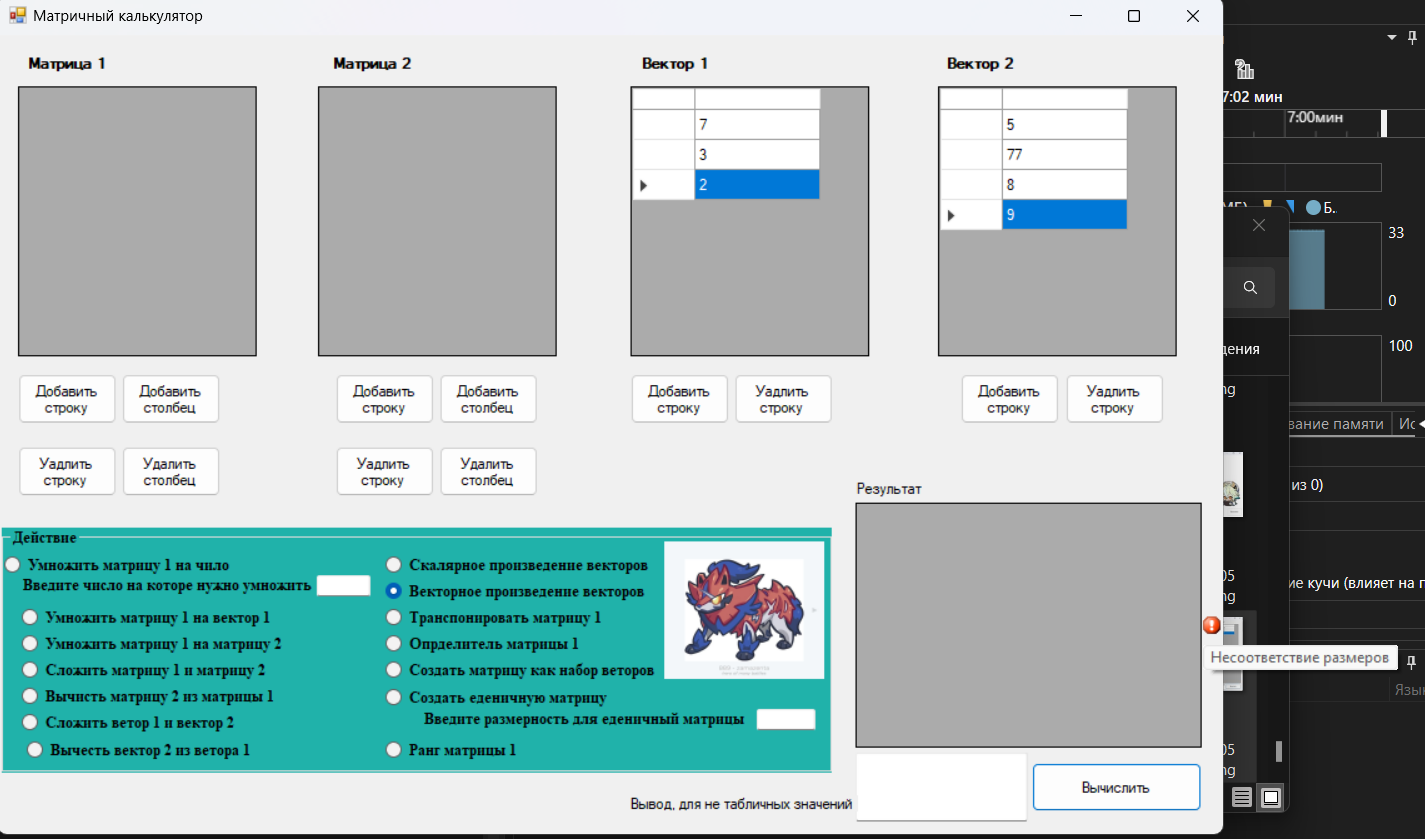
\includegraphics[scale=0.4]{Скрины/Снимок экрана 2025-01-05 134125.png}
    \caption{Окно приложения <<Матричный калькулятор>>: сообщение о некорректном вводе (<<Несоответствие размеров>>)}\label{fig:matrix-09}
\end{figure}


Полный код программы приведен в приложении~\ref{app:CD}.

\section{Файловые диалоги и работа с файлами}

\textsl{Задание.} Разработать приложение, реализующее работу с файлами.

Создано окно приложения, содержащее один элемент TextBox, один элемент Label, шесть элементов Button и два элемента DataGridView. Для отображения сообщений об ошибках в окно добавлены три элемента ErrorProvider. Для работы с файлами добавлены элементы SaveFileDialog\cite{search_7,bookc++tat} и OpenFileDialog\cite{search_8}. Вид окна представлен на рисунке~\ref{fig:file-01}.

\begin{figure}[H]
    \centering
    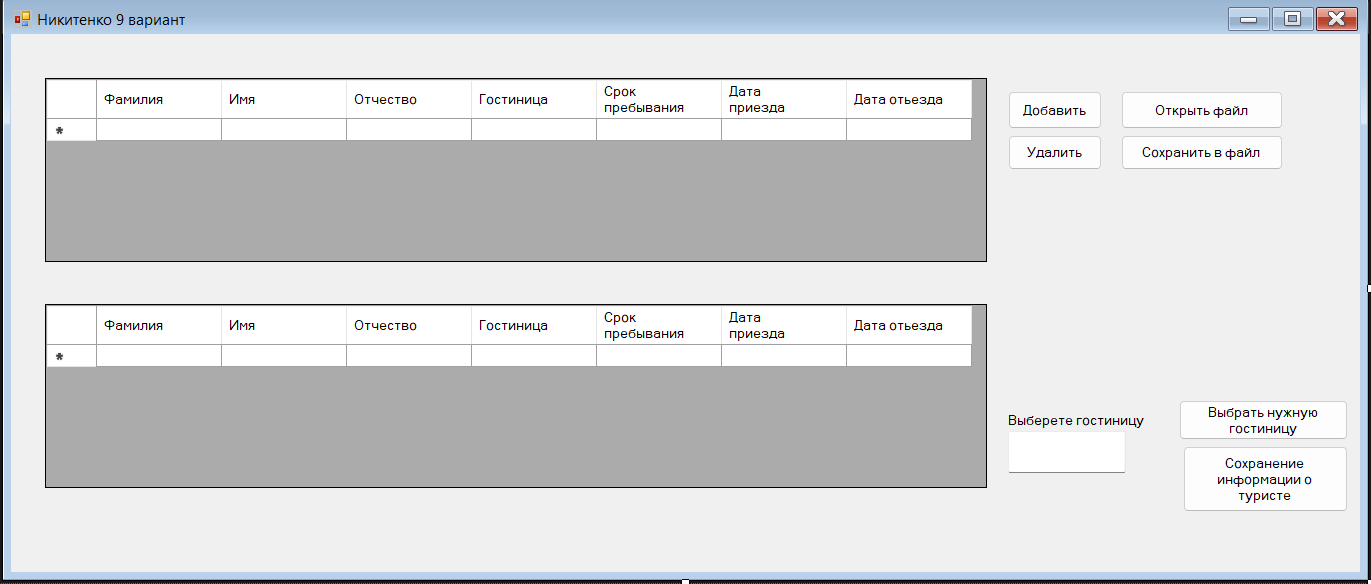
\includegraphics[scale=0.45]{Скрины/Снимок экрана 2025-01-05 134825.png}
    \caption{Окно приложения <<Никитенко 9 вариант>> открытое в конструкторе)}\label{fig:file-01}
\end{figure}

У элементов изменены значения некоторых атрибутов. Значения измененных атрибутов представлены в таблицах~\ref{tab:file-1-attr} и~\ref{tab:file-2-attr}.
\begin{table}[H]
    \small
    \caption{Значения атрибутов элементов в приложении <<Работа с файлами>>}\label{tab:file-1-attr}
    \begin{tabular}{|l|l|}\hline
    Наименование атрибута & Значение\cr\hline
    \multicolumn{2}{|l|}{Для формы}\cr\hline
    \verb"Text" & \verb"Никитенко 9 вариант"\cr\hline

    \multicolumn{2}{|l|}{Для надписи}\cr\hline
    \verb"Text" & \verb"Выбирите гостиницу"\cr\hline

    \multicolumn{2}{|l|}{Для текстового поля}\cr\hline
    \verb"(Name)" & \verb"ChoiceRace"\cr\hline

    \multicolumn{2}{|l|}{Для первой кнопки}\cr\hline
    \verb"(Name)" & \verb"Add"\cr\hline
    \verb"Text" & \verb"Добавить"\cr\hline

    \end{tabular}
\end{table}

\begin{table}[H]
    \small
    \caption{Значения атрибутов элементов в приложении <<Использование коллекций>>}\label{tab:file-2-attr}
    \begin{tabular}{|l|l|}\hline
    Наименование атрибута & Значение\cr\hline

    \multicolumn{2}{|l|}{Для второй кнопки}\cr\hline
    \verb"(Name)" & \verb"Delete"\cr\hline
    \verb"Text" & \verb"Удалить"\cr\hline

    \multicolumn{2}{|l|}{Для третьей кнопки}\cr\hline
    \verb"(Name)" & \verb"OpenFile"\cr\hline
    \verb"Text" & \verb"Открыть файл"\cr\hline

    \multicolumn{2}{|l|}{Для четвертой кнопки}\cr\hline
    \verb"(Name)" & \verb"SaveInFile"\cr\hline
    \verb"Text" & \verb"Сохранить в файл"\cr\hline

    \multicolumn{2}{|l|}{Для пятой кнопки}\cr\hline
    \verb"(Name)" & \verb"ChoiceRaceBut"\cr\hline
    \verb"Text" & \verb"Выбрать нужную гостиницу"\cr\hline

    \multicolumn{2}{|l|}{Для шестой кнопки}\cr\hline
    \verb"(Name)" & \verb"SaveInPass"\cr\hline
    \verb"Text" & \verb"Сохранение информации о туристе"\cr\hline

    \multicolumn{2}{|l|}{Для первой таблицы}\cr\hline
    \verb"(Name)" & \verb"Table1"\cr\hline
    \verb"NameColumn1" & \verb"Фамилия"\cr\hline
    \verb"NameColumn2" & \verb"Имя"\cr\hline
    \verb"NameColumn3" & \verb"Отчество"\cr\hline
    \verb"NameColumn4" & \verb"Гостиница"\cr\hline
    \verb"NameColumn5" & \verb"Срок пребывания"\cr\hline
    \verb"NameColumn6" & \verb"Дата приезда"\cr\hline
    \verb"NameColumn7" & \verb"Дата отьезда"\cr\hline

    \multicolumn{2}{|l|}{Для второй таблицы}\cr\hline
    \verb"(Name)" & \verb"Table2"\cr\hline
    \verb"NameColumn1" & \verb"Фамилия"\cr\hline
    \verb"NameColumn2" & \verb"Имя"\cr\hline
    \verb"NameColumn3" & \verb"Отчество"\cr\hline
    \verb"NameColumn4" & \verb"Гостиница"\cr\hline
    \verb"NameColumn5" & \verb"Срок пребывания"\cr\hline
    \verb"NameColumn6" & \verb"Дата приезда"\cr\hline
    \verb"NameColumn7" & \verb"Дата отьезда"\cr\hline

    \end{tabular}
\end{table}

На нажатие кнопки <<Открыть файл>> установлено выполнение следующего кода:
\inputminted[fontsize=\footnotesize]{cpp}{Файл/Open.cpp}

На нажатие кнопки <<Сохранить в файл>> установлено выполнение следующего кода:
\inputminted[fontsize=\footnotesize]{cpp}{Файл/Save.cpp}

Примеры остальных кодов приведены в приложении~\ref{app:code}.

После запуска приложения на экране появляется окно (см. рисунок~\ref{fig:file-02}).

\begin{figure}[H]
    \centering
    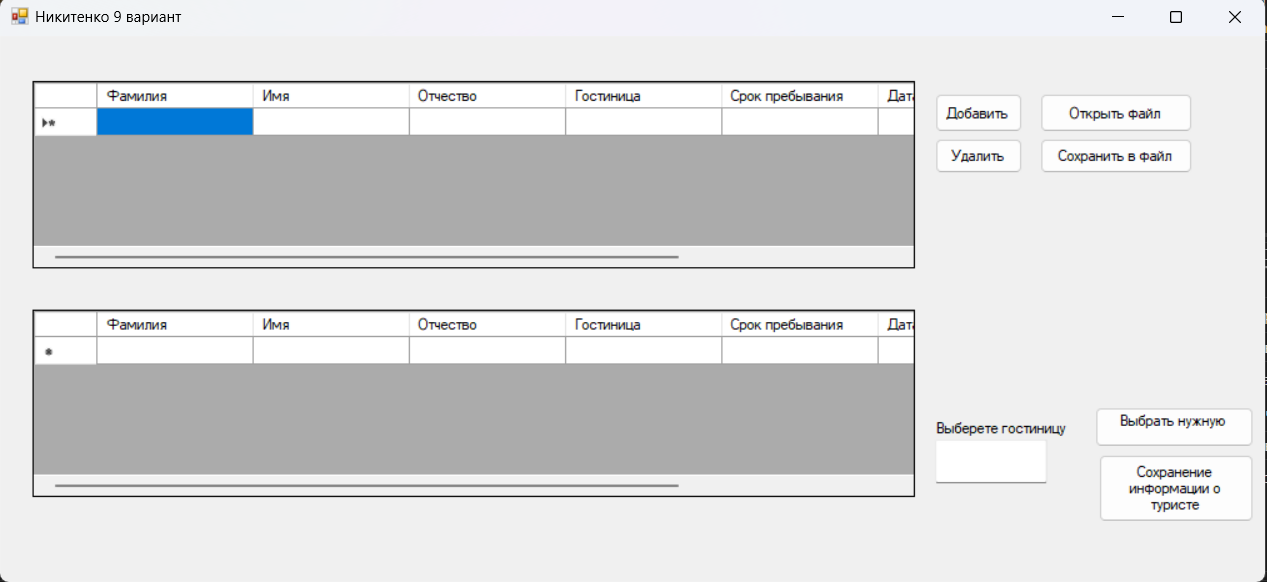
\includegraphics[scale=0.45]{Скрины/Снимок экрана 2025-01-05 142031.png}
    \caption{Окно приложения <<Работа с файлами>>: начальный запуск}\label{fig:file-02}
\end{figure}

При нажатии кнопки <<Добавить>> в первую таблицу добавляется пустая строка (см. рисунок~\ref{fig:file-03}).

\begin{figure}[H]
    \centering
    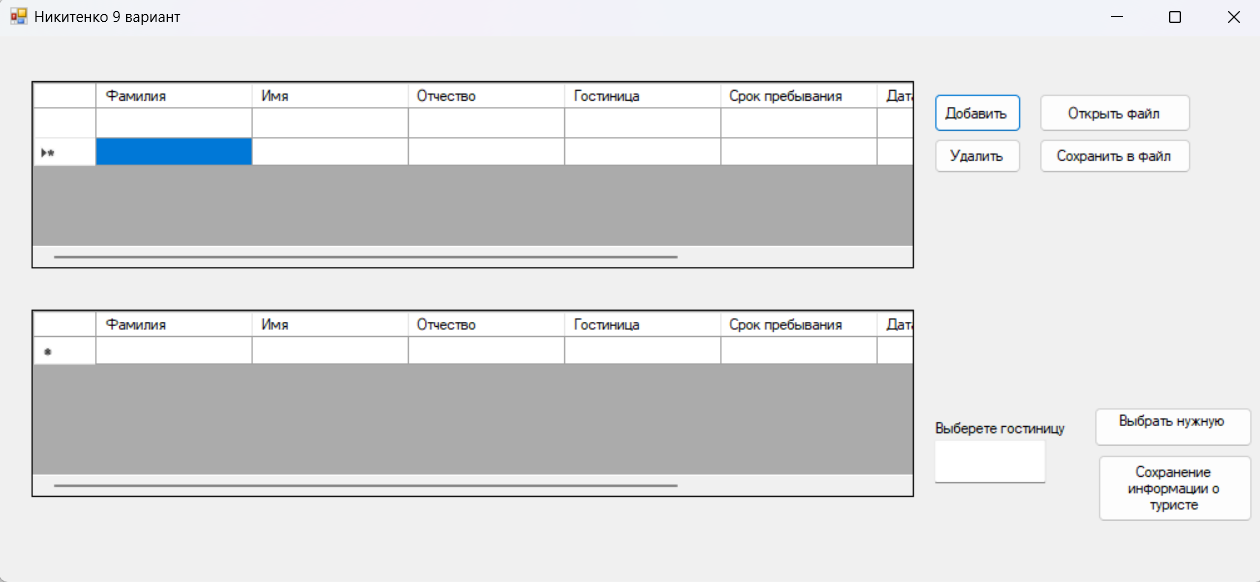
\includegraphics[scale=0.45]{Скрины/Снимок экрана 2025-01-05 142140.png}
    \caption{Окно приложения <<Работа с файлами>>: корректное добавление строки}\label{fig:file-03}
\end{figure}

При нажатии кнопки <<Удалить>> из первой таблицы удаляется выбранная строка (см. рисунок~\ref{fig:file-04}).

\begin{figure}[H]
    \centering
    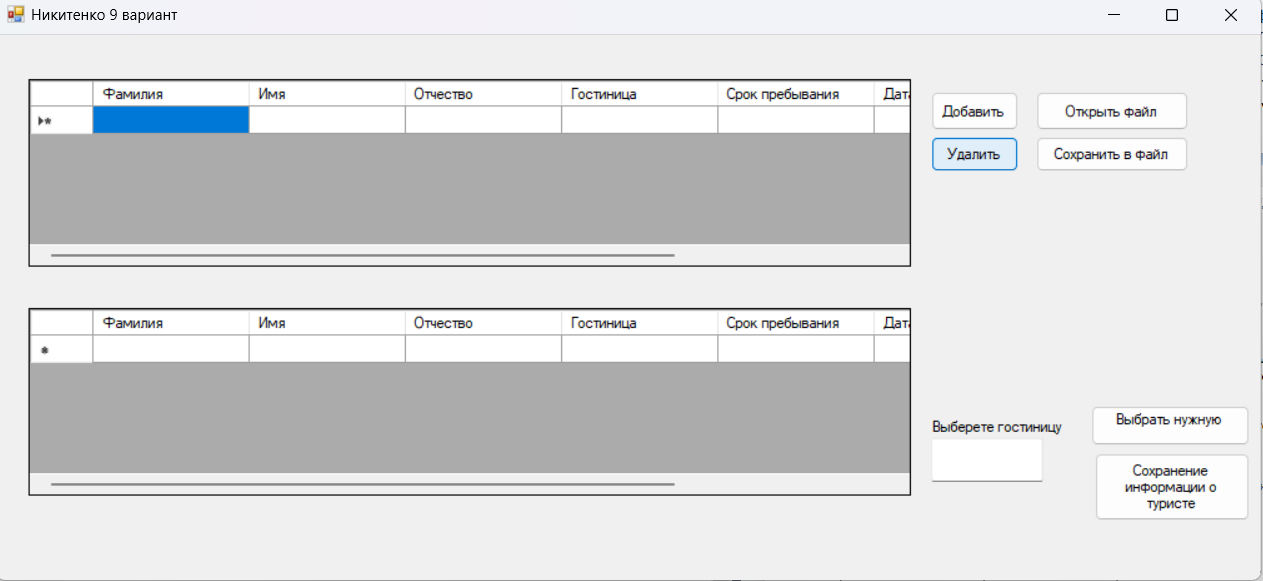
\includegraphics[scale=0.45]{Скрины/Снимок экрана 2025-01-05 142205.png}
    \caption{Окно приложения <<Работа с файлами>>: корректное удаление строки}\label{fig:file-04}
\end{figure}

При нажатии кнопки <<Открыть файл>> вызывается окно открытия файла (см. рисунок~\ref{fig:file-05}).

\begin{figure}[H]
    \centering
    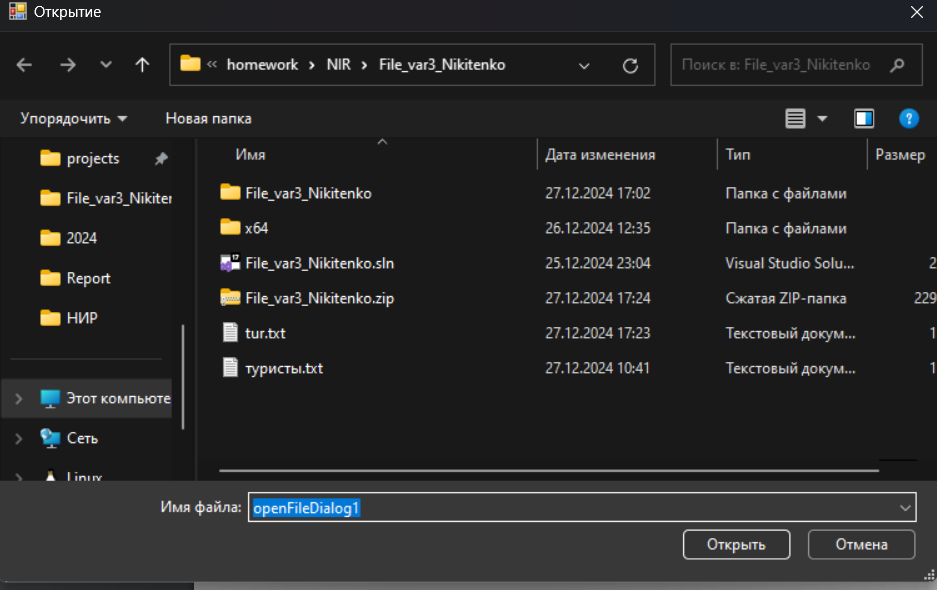
\includegraphics[scale=0.45]{Скрины/Снимок экрана 2025-01-05 142255.png}
    \caption{Окно приложения <<Работа с файлами>>: корректное открытие файла}\label{fig:file-05}
\end{figure}

При нажатии кнопки <<Выбрать нужную гостиницу>> и вводе корректного названия гостинице в соответствующее поле во второй таблице появляются данные о туристе в этой гостинице (см. рисунок~\ref{fig:file-06}).

\begin{figure}[H]
    \centering
    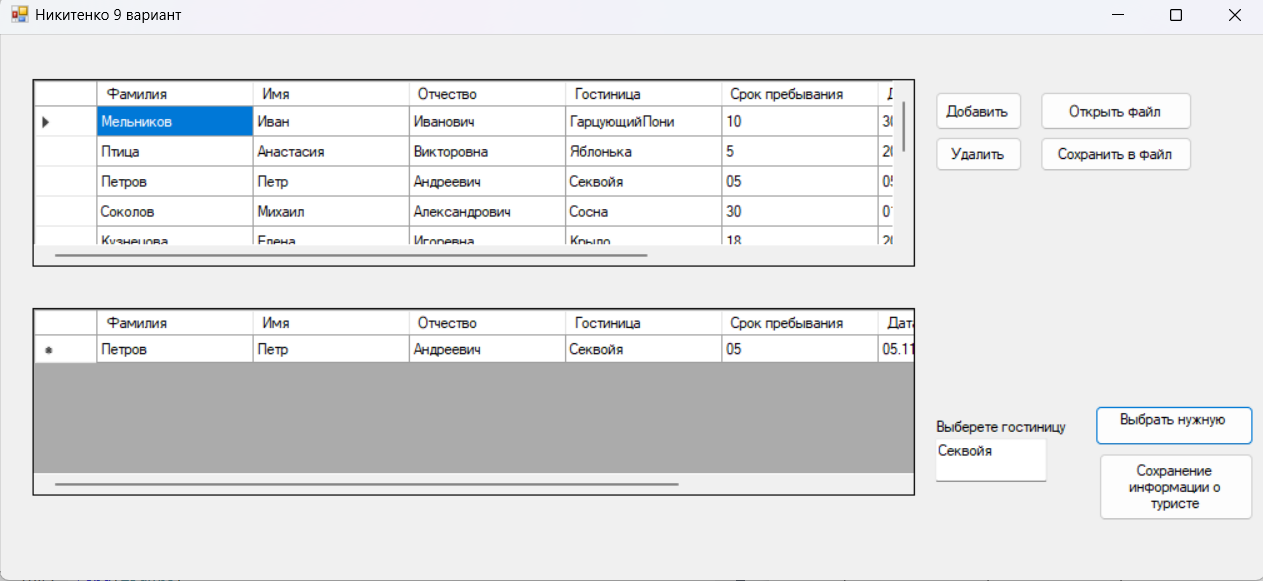
\includegraphics[scale=0.45]{Скрины/Снимок экрана 2025-01-05 142342.png}
    \caption{Окно приложения <<Работа с файлами>>: корректный выбор гостиницы и вывод данных}\label{fig:file-06}
\end{figure}

При нажатии кнопки <<Сохранение информации о туристе>> открывается окно для сохранения файла с выбранными туристами (см. рисунок~\ref{fig:file-07}).

\begin{figure}[H]
    \centering
    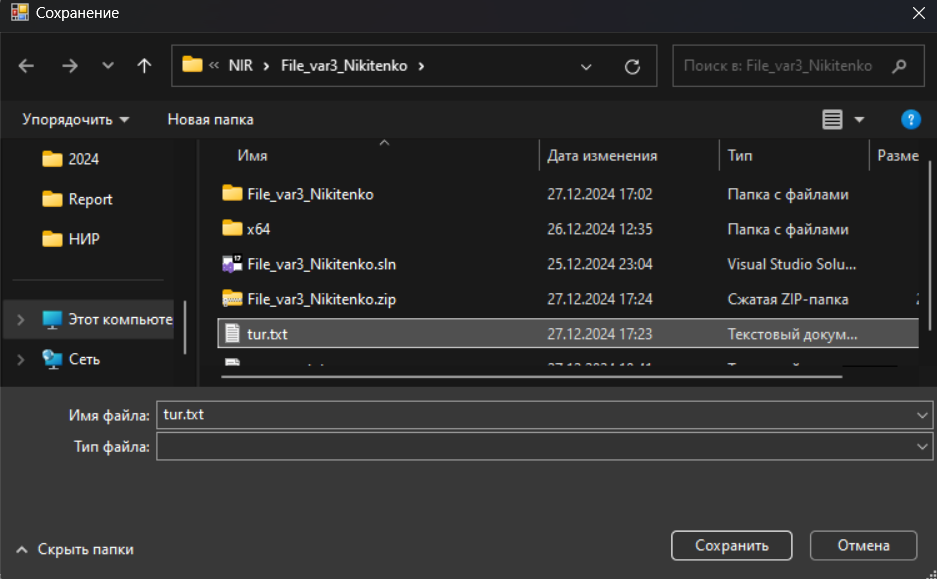
\includegraphics[scale=0.45]{Скрины/Снимок экрана 2025-01-05 142412.png}
    \caption{Окно приложения <<Работа с файлами>>: корректное сохранение файла с выбранными туристами}\label{fig:file-07}
\end{figure}

При нажатии кнопки <<Сохранить в файл>> открывается окно для сохранения файла со всеми туристами (см. рисунок~\ref{fig:file-08}).

\begin{figure}[H]
    \centering
    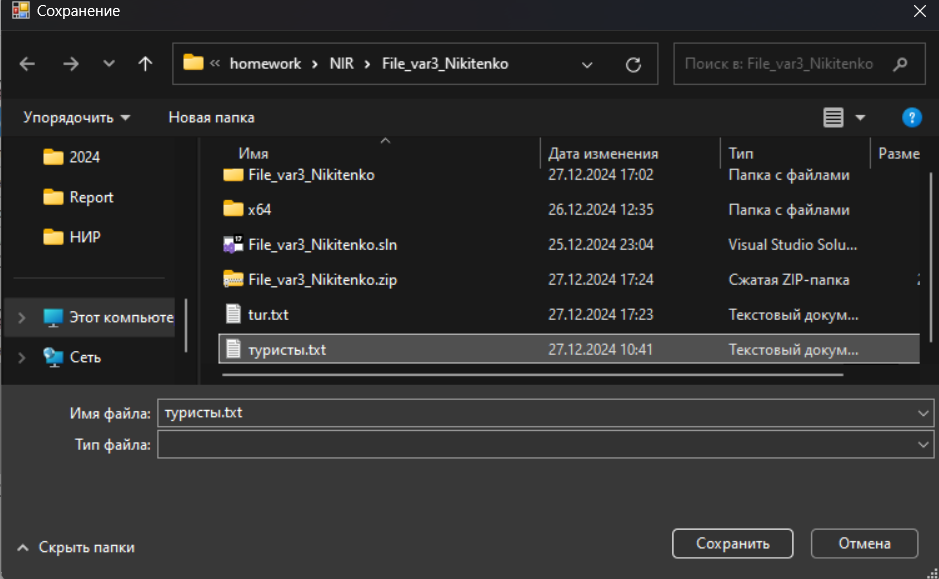
\includegraphics[scale=0.45]{Скрины/Снимок экрана 2025-01-05 142525.png}
    \caption{Окно приложения <<Работа с файлами>>: корректное сохранение файла со всеми туристами}\label{fig:file-08}
\end{figure}

При нажатии кнопки <<Открыть файл>> и закрытии окна без выбранного файла возникает сообщение об ошибке (см. рисунок~\ref{fig:file-09}).

\begin{figure}[H]
    \centering
    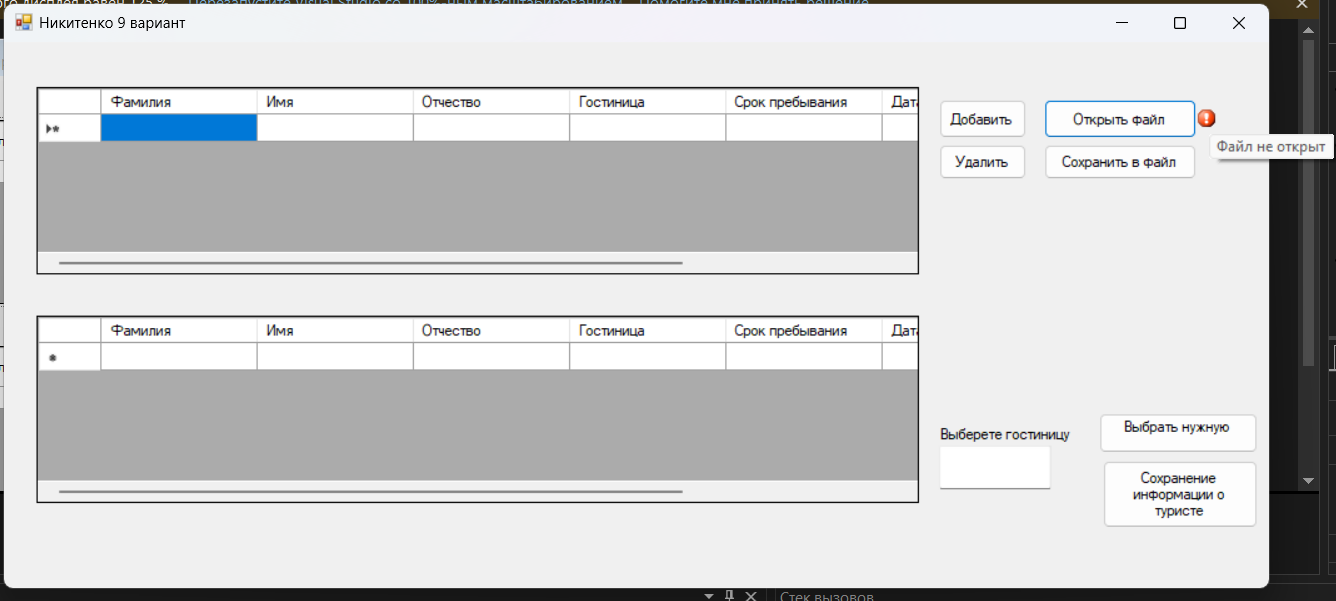
\includegraphics[scale=0.45]{Скрины/Снимок экрана 2025-01-05 142621.png}
    \caption{Окно приложения <<Работа с файлами>>: сообщение о некорректном открытии файла (<<Файл не открыт>>)}\label{fig:file-09}
\end{figure}

При нажатии кнопки <<Выбрать нужную гостиницу>> и пустом поле с названием гостинцы возникает сообщение об ошибке (см. рисунок~\ref{fig:file-10}).

\begin{figure}[H]
    \centering
    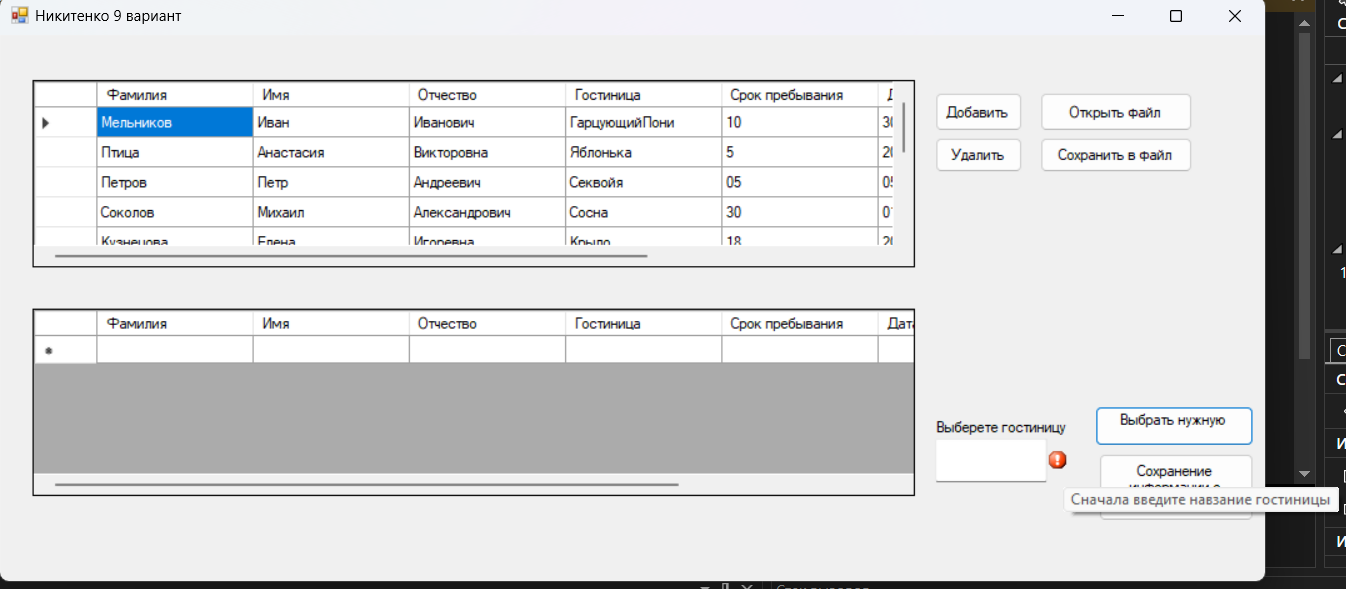
\includegraphics[scale=0.45]{Скрины/Снимок экрана 2025-01-05 142730.png}
    \caption{Окно приложения <<Работа с файлами>>: сообщение о некорректном выборе рейса (<<Сначала введите название гостиницы>>)}\label{fig:file-10}
\end{figure}

Полный код программы приведен в приложении~\ref{app:CD}.

\section{Использование коллекций в Windows Forms}

\textsl{Задание.} Разработать приложение, реализующее работу с очередью\cite{bookc++bern}.

Создано окно приложения, содержащее пять элементов TextBox, четыре элемента Label и шесть элементов Button. Для отображения сообщений об ошибках в окно добавлены три элемента ErrorProvider. Вид окна представлен на рисунке~\ref{fig:queue-01}.

\begin{figure}[H]
    \centering
    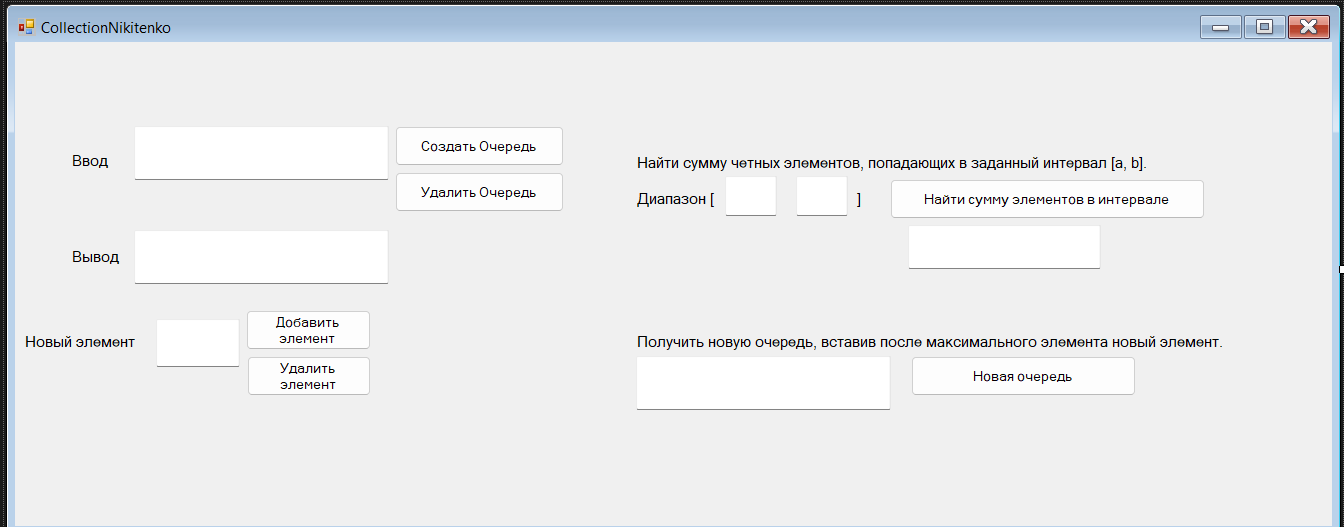
\includegraphics[scale=0.5]{Скрины/Снимок экрана 2025-01-05 203620.png}
    \caption{Окно приложения <<CollectionNikitenko>> открытое в конструкторе}\label{fig:queue-01}
\end{figure}

У элементов изменены значения некоторых атрибутов. Значения измененных атрибутов представлены в таблицах~\ref{tab:queue-01-attr} и~\ref{tab:queue-02-attr}.
\begin{table}[H]
    \small
    \caption{Значения атрибутов элементов в приложении <<Использование коллекций>>}\label{tab:queue-01-attr}
    \begin{tabular}{|l|l|}\hline
    Наименование атрибута & Значение\cr\hline
    \multicolumn{2}{|l|}{Для формы}\cr\hline
    \verb"Text" & \verb"CollectionNikitenko"\cr\hline

    \multicolumn{2}{|l|}{Для первой надписи}\cr\hline
    \verb"Text" & \verb"Ввод"\cr\hline

    \multicolumn{2}{|l|}{Для второй надписи}\cr\hline
    \verb"Text" & \verb"Вывод"\cr\hline

    \multicolumn{2}{|l|}{Для третьей надписи}\cr\hline
    \verb"Text" & \verb"Новый элемент "\cr\hline
    \end{tabular}
\end{table}

\begin{table}[H]
    \small
    \caption{Значения атрибутов элементов в приложении <<Использование коллекций>>}\label{tab:queue-02-attr}
    \begin{tabular}{|l|l|}\hline
    Наименование атрибута & Значение\cr\hline

    \multicolumn{2}{|l|}{Для четвертой надписи}\cr\hline
    \verb"Text" & \verb"Получить новую очередь,"\\ 
    &\verb"вставив после максимального элемента новый элемент."\cr\hline
   
     \multicolumn{2}{|l|}{Для пятой надписи}\cr\hline
    \verb"Text" & \verb"Диапазон."\cr\hline

     \multicolumn{2}{|l|}{Для шестой надписи}\cr\hline
    \verb"Text" & \verb"Найти сумму четных элементов,"\\ 
    &\verb"попадающих в заданный интервал [a, b]."\cr\hline

    \multicolumn{2}{|l|}{Для первого текстового поля}\cr\hline
    \verb"(Name)" & \verb"InPutQu"\cr\hline

    \multicolumn{2}{|l|}{Для второго текстового поля}\cr\hline
    \verb"(Name)" & \verb"OutPutQu"\cr\hline

    \multicolumn{2}{|l|}{Для третьего текстового поля}\cr\hline
    \verb"(Name)" & \verb"NewElIn"\cr\hline

    \multicolumn{2}{|l|}{Для четвертого текстового поля}\cr\hline
    \verb"(Name)" & \verb"a"\cr\hline

    \multicolumn{2}{|l|}{Для пятого текстового поля}\cr\hline
    \verb"(Name)" & \verb"b"\cr\hline

    \multicolumn{2}{|l|}{Для шестого текстового поля}\cr\hline
    \verb"(Name)" & \verb"ChotElem"\cr\hline

    \multicolumn{2}{|l|}{Для седьмого текстового поля}\cr\hline
    \verb"(Name)" & \verb"NewQOut"\cr\hline

    \multicolumn{2}{|l|}{Для первой кнопки}\cr\hline
    \verb"(Name)" & \verb"CreateQ"\cr\hline
    \verb"Text" & \verb"Создать очередь"\cr\hline

    \multicolumn{2}{|l|}{Для второй кнопки}\cr\hline
    \verb"(Name)" & \verb"DeleteQu"\cr\hline
    \verb"Text" & \verb"Удалить очередь"\cr\hline

    \multicolumn{2}{|l|}{Для третьей кнопки}\cr\hline
    \verb"(Name)" & \verb"AddEl"\cr\hline
    \verb"Text" & \verb"Добавить элемент"\cr\hline

    \multicolumn{2}{|l|}{Для четвертой кнопки}\cr\hline
    \verb"(Name)" & \verb"DeleteEl"\cr\hline
    \verb"Text" & \verb"Удалить элемент"\cr\hline

    \multicolumn{2}{|l|}{Для пятой кнопки}\cr\hline
    \verb"(Name)" & \verb"Interval"\cr\hline
    \verb"Text" & \verb"Найти сумму элементов в интервале"\cr\hline

    \multicolumn{2}{|l|}{Для шестой кнопки}\cr\hline
    \verb"(Name)" & \verb"NewQ"\cr\hline
    \verb"Text" & \verb"Новая очередь"\cr\hline

    \end{tabular}
\end{table}

На нажатие кнопки <<Создать очередь>> установлено выполнение следующего кода:
\inputminted[fontsize=\footnotesize]{cpp}{Колекции/CreateQ.cpp}

На нажатие кнопки <<Найти сумму элементов в интервале>> установлено выполнение следующего кода:
\inputminted[fontsize=\footnotesize]{cpp}{Колекции/Interval.cpp}

Примеры остальных кодов приведены в приложении~\ref{app:code}.

После запуска приложения на экране появляется окно (см. рисунок~\ref{fig:queue-02}).

\begin{figure}[H]
    \centering
    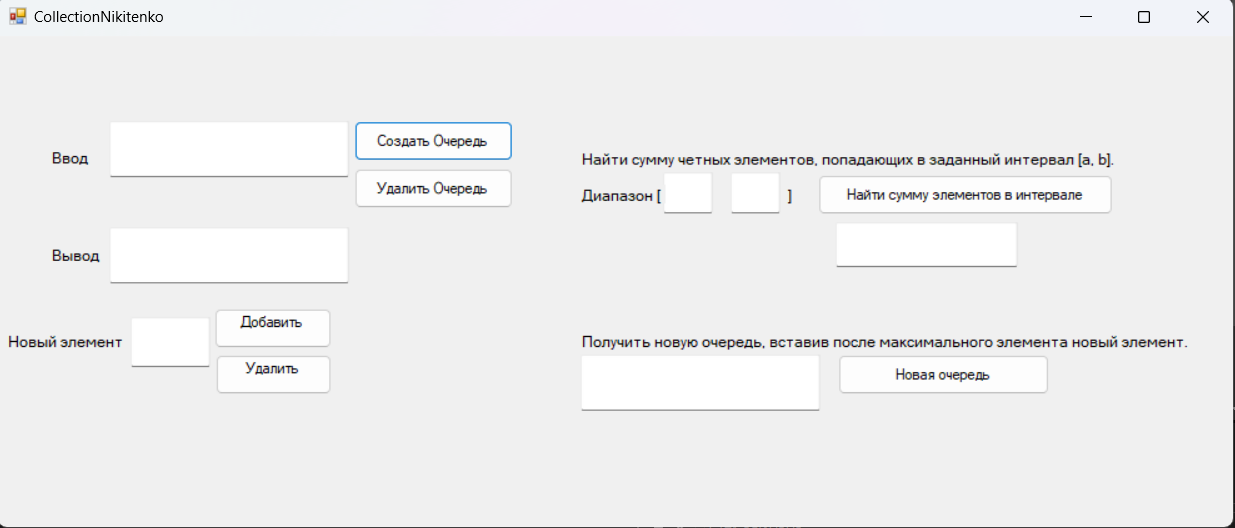
\includegraphics[scale=0.5]{Скрины/Снимок экрана 2025-01-05 205837.png}
    \caption{Окно приложения <<CollectionNikitenko>>: начальный запуск}\label{fig:queue-02}
\end{figure}

При вводе целых чисел в поле для ввода и нажатии кнопок <<Создать очередь>>, <<Новая очередь>>, <<Найти сумму элементов в интервале>> в поле вывода очереди записываются введенные числа, в поле для новой очереди записывается очередь, потом находится максимальный элемент и после него вставляется новый элемент и после введения диапазона записывается сумма элементов попавших в этот диапазон (см. рисунок~\ref{fig:queue-03}).

\begin{figure}[H]
    \centering
    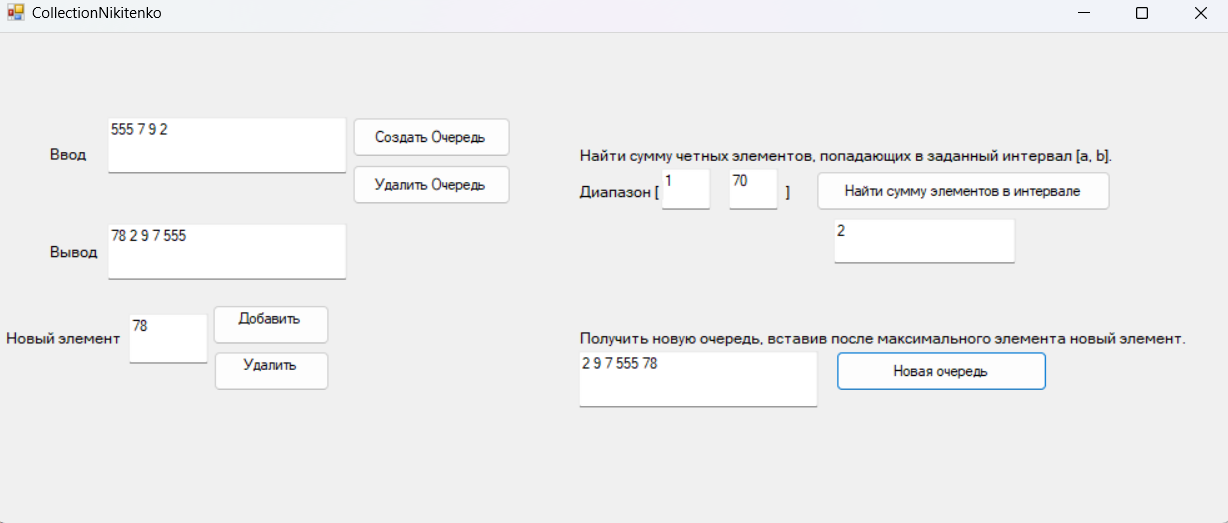
\includegraphics[scale=0.5]{Скрины/Снимок экрана 2025-01-05 212210.png}
    \caption{Окно приложения <<CollectionNikitenko>>: корректное создание очереди и выполнение указанных действий}\label{fig:queue-03}
\end{figure}

При нажатии кнопки <<Удалить очередь>> выполняется удаление очереди (см. рисунок~\ref{fig:queue-04}).

\begin{figure}[H]
    \centering
    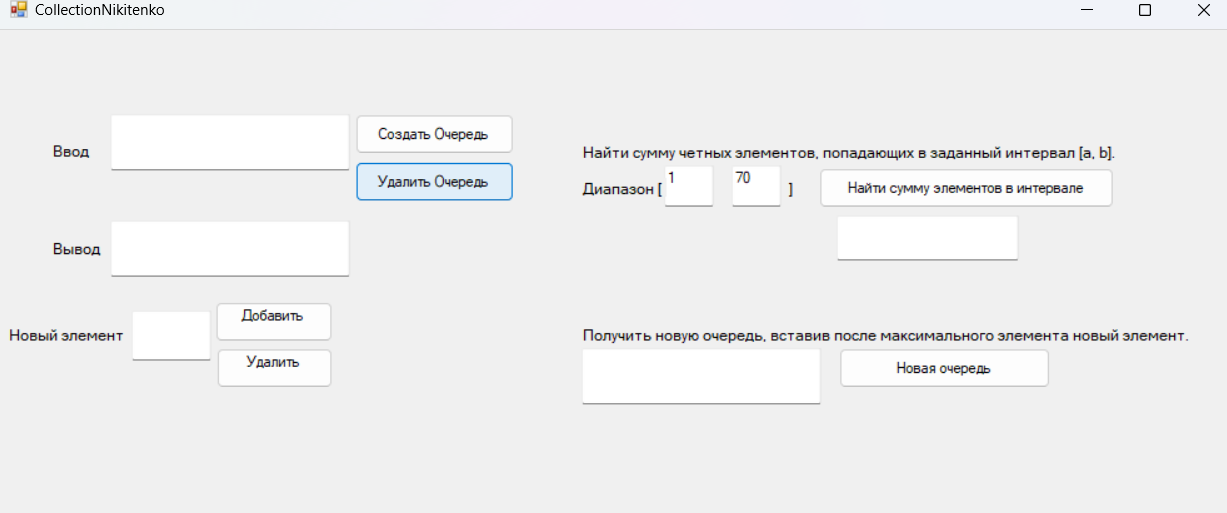
\includegraphics[scale=0.5]{Скрины/Снимок экрана 2025-01-05 212248.png}
    \caption{Окно приложения <<Использование коллекций>>: корректное удаление очереди}\label{fig:queue-04}
\end{figure}

При нажатии на кнопку <<Добавить элемент>> и вводе целого числа в соответствующее поле в поле вывода очереди записывается новый элемент (см. рисунок~\ref{fig:queue-05}).

\begin{figure}[H]
    \centering
    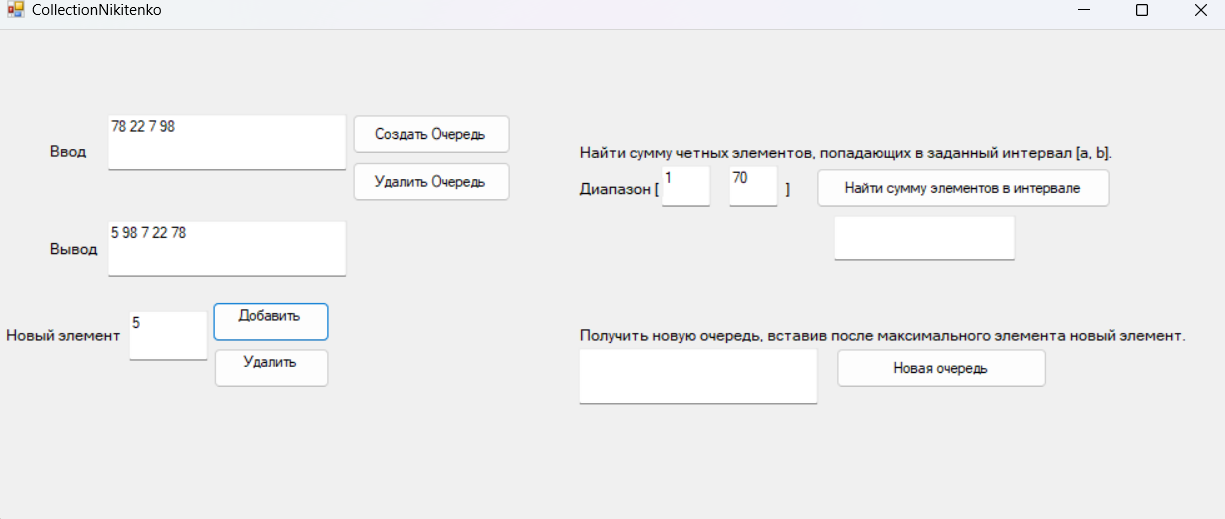
\includegraphics[scale=0.5]{Скрины/Снимок экрана 2025-01-05 212325.png}
    \caption{Окно приложения <<Использование коллекций>>: корректное добавление нового элемента}\label{fig:queue-05}
\end{figure}

При нажатии кнопки <<Добавить элемент>> и отсутствии целого числа в соответствующем поле выводится сообщение об ошибке (см. рисунок~\ref{fig:queue-06}).

\begin{figure}[H]
    \centering
    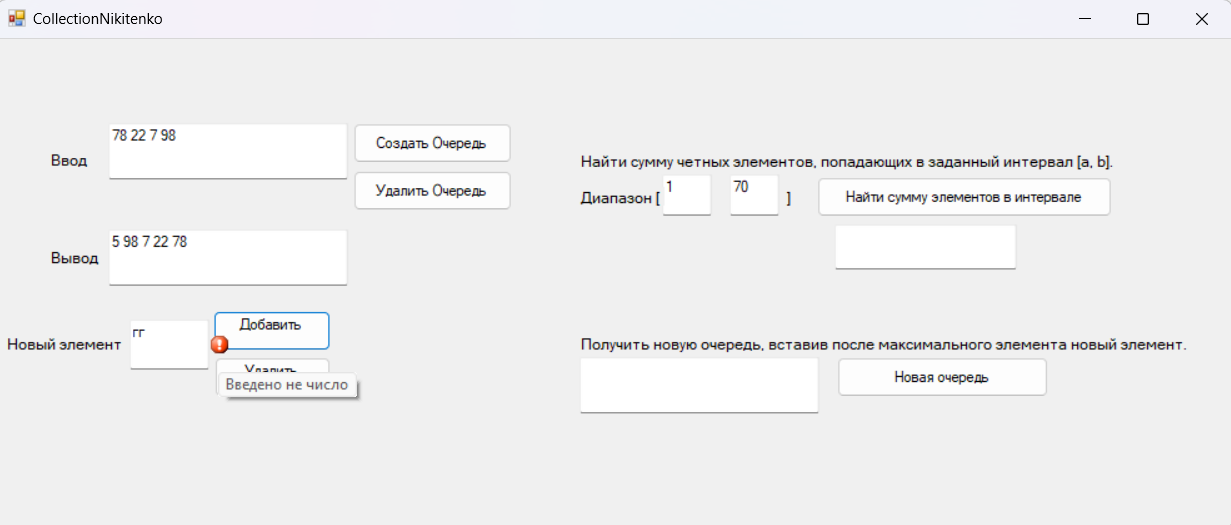
\includegraphics[scale=0.5]{Скрины/Снимок экрана 2025-01-05 212418.png}
    \caption{Окно приложения <<Использование коллекций>>: сообщение о некорректном вводе (<<Введено не число>>)}\label{fig:queue-06}
\end{figure}

При нажатии кнопки <<Найти сумму элементов в интервале>> и отсутствии четных элементов в данном интервале выводиться сообщение о том что таких элементов нет (см. рисунок~\ref{fig:queue-07}).

\begin{figure}[H]
    \centering
    \includegraphics[scale=0.5]{Скрины/Снимок экрана 2025-01-05 212905.png}
    \caption{Окно приложения <<Использование коллекций>>: сообщение о об отсутствии элементов (<<Таких элементов нет>>)}\label{fig:queue-07}
\end{figure}


Полный код программы приведен в приложении~\ref{app:CD}.

\section{Приложение ТЕСТ}

\textsl{Задание.} Разработать приложение для тестирования.

Создано окно приложения, содержащее один элемент TextBox, шесть элементов Label, четыре элемента Button, три элемента CheckBox и три элемента RadioButton. Вид окна представлен на рисунке~\ref{fig:test-01}.

\begin{figure}[H]
    \centering
    \includegraphics[scale=0.7]{Скрины/Снимок экрана 2025-01-05 213031.png}
    \caption{Окно приложения <<Тест>> открытое в конструкторе)}\label{fig:test-01}
\end{figure}

У элементов изменены значения некоторых атрибутов. Значения измененных атрибутов представлены в таблицах~\ref{tab:test-1-attr} и~\ref{tab:test-2-attr}.
\begin{table}[H]
    \small
    \caption{Значения атрибутов элементов в приложении <<Тест>>}\label{tab:test-1-attr}
    \begin{tabular}{|l|l|}\hline
    Наименование атрибута & Значение\cr\hline
    \multicolumn{2}{|l|}{Для формы}\cr\hline
    \verb"Text" & \verb"ДИНОЗАВРИКИ"\cr\hline

    \multicolumn{2}{|l|}{Для текстового поля}\cr\hline
    \verb"Visible" & \verb"False"\cr\hline

    \multicolumn{2}{|l|}{Для первого переключателя}\cr\hline
    \verb"Visible" & \verb"False"\cr\hline

    \multicolumn{2}{|l|}{Для второго переключателя}\cr\hline
    \verb"Visible" & \verb"False"\cr\hline

    \multicolumn{2}{|l|}{Для третьего переключателя}\cr\hline
    \verb"Visible" & \verb"False"\cr\hline

    \multicolumn{2}{|l|}{Для первой надписи}\cr\hline
    \verb"(Name)" & \verb"lblNum1"\cr\hline
    \verb"Text" & \verb"Вопрос №"\cr\hline
    \verb"Visible" & \verb"False"\cr\hline

    \end{tabular}
\end{table}

\begin{table}[H]
    \small
    \caption{Значения атрибутов элементов в приложении <<Использование коллекций>>}\label{tab:test-2-attr}
    \begin{tabular}{|l|l|}\hline
    Наименование атрибута & Значение\cr\hline

    \multicolumn{2}{|l|}{Для первого флажка}\cr\hline
    \verb"Visible" & \verb"False"\cr\hline

    \multicolumn{2}{|l|}{Для второго флажка}\cr\hline
    \verb"Visible" & \verb"False"\cr\hline

    \multicolumn{2}{|l|}{Для третьего флажка}\cr\hline
    \verb"Visible" & \verb"False"\cr\hline

    \multicolumn{2}{|l|}{Для второй надписи}\cr\hline
    \verb"(Name)" & \verb"lblNum2"\cr\hline
    \verb"Visible" & \verb"False"\cr\hline

    \multicolumn{2}{|l|}{Для третьей надписи}\cr\hline
    \verb"(Name)" & \verb"lblQuestion"\cr\hline
    \verb"Visible" & \verb"False"\cr\hline

    \multicolumn{2}{|l|}{Для четвертой надписи}\cr\hline
    \verb"(Name)" & \verb"lblAnswer"\cr\hline
    \verb"Visible" & \verb"False"\cr\hline

    \multicolumn{2}{|l|}{Для пятой надписи}\cr\hline
    \verb"(Name)" & \verb"lblTrue"\cr\hline
    \verb"Text" & \verb"Количество правильных ответов:"\cr\hline
    \verb"Visible" & \verb"False"\cr\hline

    \multicolumn{2}{|l|}{Для шестой надписи}\cr\hline
    \verb"(Name)" & \verb"lblFalse"\cr\hline
    \verb"Text" & \verb"Количество неправильных ответов:"\cr\hline
    \verb"Visible" & \verb"False"\cr\hline

    \multicolumn{2}{|l|}{Для первой кнопки}\cr\hline
    \verb"(Name)" & \verb"btnStart"\cr\hline
    \verb"Text" & \verb"НАЧАТЬ"\cr\hline

    \multicolumn{2}{|l|}{Для второй кнопки}\cr\hline
    \verb"(Name)" & \verb"btnCheck"\cr\hline
    \verb"Text" & \verb"Проверить ответ"\cr\hline
    \verb"Visible" & \verb"False"\cr\hline

    \multicolumn{2}{|l|}{Для третьей кнопки}\cr\hline
    \verb"(Name)" & \verb"btnNext"\cr\hline
    \verb"Text" & \verb"Следующий вопрос"\cr\hline
    \verb"Visible" & \verb"False"\cr\hline

    \multicolumn{2}{|l|}{Для четвертой кнопки}\cr\hline
    \verb"(Name)" & \verb"btnRes"\cr\hline
    \verb"Text" & \verb"Завершить тест"\cr\hline
    \verb"Visible" & \verb"False"\cr\hline

    \end{tabular}
\end{table}

На нажатие кнопки <<НАЧАТЬ>> установлено выполнение следующего кода:
\inputminted[fontsize=\footnotesize]{cpp}{Тест/Start.cpp}

На нажатие кнопки <<Проверить ответ>> установлено выполнение следующего кода:
\inputminted[fontsize=\footnotesize]{cpp}{Тест/Check.cpp}

На нажатие кнопки <<Завершить тест>> установлено выполнение следующего кода:
\inputminted[fontsize=\footnotesize]{cpp}{Тест/Complite.cpp}

Примеры остальных кодов приведены в приложении~\ref{app:code}.

После запуска приложения на экране появляется окно (см. рисунок~\ref{fig:test-02}).

\begin{figure}[H]
    \centering
    \includegraphics[scale=0.7]{Скрины/Снимок экрана 2025-01-05 213834.png}
    \caption{Окно приложения <<Тест>>: начальный запуск}\label{fig:test-02}
\end{figure}

При нажатии на кнопку <<НАЧАТЬ>> некоторые элементы формы становятся видимыми и в случайном порядке появляются вопросы и варианты ответа на них (см. рисунок~\ref{fig:test-03}).

\begin{figure}[H]
    \centering
    \includegraphics[scale=0.7]{Скрины/Снимок экрана 2025-01-05 213834.png}
    \caption{Окно приложения <<Тест>>: начало тестирования}\label{fig:test-03}
\end{figure}

При выборе ответа и нажатии на кнопку <<Проверить ответ>> появляется сообщение и правильности ответа, кнопка <<Следующий вопрос>> и запрещается редактировать ответ (см. рисунок~\ref{fig:test-04}).

\begin{figure}[H]
    \centering
    \includegraphics[scale=0.7]{Скрины/Снимок экрана 2025-01-05 213922.png}
    \caption{Окно приложения <<Тест>>: ответы на вопросы}\label{fig:test-04}
\end{figure}

Когда вопросы заканчиваются, появляется кнопка <<Завершить тест>> (см. рисунок~\ref{fig:test-05}).

\begin{figure}[H]
    \centering
    \includegraphics[scale=0.7]{Скрины/Снимок экрана 2025-01-05 214141.png}
    \caption{Окно приложения <<Тест>>: завершение теста}\label{fig:test-05}
\end{figure}

При нажатии кнопки <<Завершить тест>> появляется информация с результатами прохождения теста (см. рисунок~\ref{fig:test-06}).

\begin{figure}[H]
    \centering
    \includegraphics[scale=0.7]{Скрины/Снимок экрана 2025-01-05 214040.png}
    \caption{Окно приложения <<Тест>>: результаты тестирования}\label{fig:test-06}
\end{figure}

Полный код программы приведен в приложении~\ref{app:CD}.

% Раздел "Заключение"
\conclusion
В ходе практики было реализовано несколько приложений на языке C++ в среде Microsoft Visual Studio с целью закрепления навыков построения оконного интерфейса. На практике разработаны приложения, содержащие такие элементы интерфейса как \verb"TextBox", \verb"Label", \verb"Button", \verb"DataGridView", \linebreak \verb"OpenFileDialog", \verb"SaveFileDialog", \verb"ErrorProvider".

    \bibliographystyle{gost780uv.bst}
    \bibliography{thesis}
    
    \appendix
\section{Примеры кода}\label{app:code} 

\subsection*{Обработка табличных данных. Часть 1}

На нажатие кнопки «Среднее арифметическое» установлено выполнение следующего кода:
\inputminted[fontsize=\footnotesize]{cpp}{Код/Sred.cpp}

На нажатие кнопки «Номера нечетных элементов» установлено выполнение следующего кода:
\inputminted[fontsize=\footnotesize]{cpp}{Код/Nechet.cpp}

\subsection*{Обработка табличных данных. Часть 2}
На нажатие кнопки «Выполнить» установлено выполнение следующего кода:\inputminted[fontsize=\footnotesize]{cpp}{КодТаблица2/Execute.cpp}

\subsection*{Файловые диалоги и работа с файлами}
На нажатие кнопки <<Выбрать нужную гостиницу>> установлено выполнение следующего кода:
\inputminted[fontsize=\footnotesize]{cpp}{Файл/Ch.cpp}

На нажатие кнопки <<Сохранить информацию о туристе>> установлено выполнение следующего кода:
\inputminted[fontsize=\footnotesize]{cpp}{Файл/SaveChoice.cpp}

\subsection*{Использование коллекций в Windows Forms}
На нажатие кнопки <<Добавить элемент>> установлено выполнение следующего кода:
\inputminted[fontsize=\footnotesize]{cpp}{Колекции/Add.cpp}

На нажатие кнопки <<Новая очередь>> установлено выполнение следующего кода:
\inputminted[fontsize=\footnotesize]{cpp}{Колекции/NewQu.cpp}



\subsection*{Приложение «ТЕСТ»}
На нажатие кнопки <<Следующий вопрос>> установлено выполнение следующего кода:
\inputminted[fontsize=\footnotesize]{cpp}{Тест/Next.cpp}



\section{CD-диск с отчетом о выполненной работе}\label{app:CD}
На приложенном диске можно ознакомиться со следующими файлами:
\begin{description}
\item[Папка \texttt{Otchet}] "---   \LaTeX- вариант отчета о практике;
\item[Папка \texttt{Factorial}] "--- задание \No 1;
\item[Папка \texttt{Simple}] "---  задание \No 2, вариант \No 12;
\item[Папка \texttt{Recursion}] "--- задание \No 3, вариант \No 3;
\item[Папка \texttt{Table1}] "--- задание \No 4, вариант \No 2;
\item[Папка \texttt{Table2}] "--- задание \No 5, вариант \No 6;
\item[Папка \texttt{Matrix}] "--- задание \No 6, вариант;
\item[Папка \texttt{Collections}] "--- задание \No 7, вариант \No 8;
\item[Папка \texttt{File}] "--- задание \No 8, вариант \No 9;
\item[Папка \texttt{Test}] "--- задание \No 9;

\item[\texttt{Otchet.pdf}] "--- отчет о практике.
\end{description}
    
    
    
    
\end{document}